In this section, we describe the different experiments that were conducted in
order to evaluate and compare the algorithms described in Sections
\ref{chap:wfd}, \ref{chap:ffd} and \ref{chap:maint}. In Section
\ref{section:experiments_background} we describe the settings of the testing
environment. In Section \ref{section:experiments_overall_compare} we compare 
all discussed frontier detection algorithms. In Section
\ref{section:experiments_ffd_finer_resolution} we examine \FFD algorithm in a
finer resolution and test different aspects that might affect its performance.

\subsection{Background}
\label{section:experiments_background}
We have fully implemented \WFD, \WFDINC, \WFDIP and \FFD and performed testings
on data obtained from the Robotics Data Set Repository (Radish) \cite{Radish}. 
%We used \WFD without the suggested speed-up feature (Section
%\ref{section:wfd_speedup}), in order to compare all algorithms fairly. 
Figure \ref{fig:testing_environments} shows the environments used for
the evaluation. \WFD, \WFDINC, \WFDIP and \FFD were compared with a \SOTA (state-of-the-art)
frontier detection algorithm, due to Wurm\footnote{We thank Kai M. Wurm and Wolfram Burgard for
providing us with their own implementation of state-of-the-art frontier
detection algorithm.} and Burgard~\cite{wurm08iros,kai_2010_email}.

To evaluate the algorithms, we integrated them into a single-robot exploration
system. The system is based on GMapping, an open-source SLAM implementation
\cite{grisetti05icra, grisetti07tro}.
We integrated our code into the 
\emph{ScanMatcher} component which is contained inside \emph{gsp thread} (Grid
SLAM Processor). At the time that a new MapEvent is raised, all frontier
detection algorithms are executed according to current world state. Execution
times are measured by Linux system-call \emph{getrusage}, which measures the
CPU-process time.

We used several environments taken from Radish \cite{Radish}:
\begin{description}
  \item[(A)] Cartesium Building, University of Bremen
  \item[(B)] Freiburg, Building 079
  \item[(C)] Outdoor dataset recorded at the University of
  Freiburg
  \item[(D)] 3rd Floor of MIT CSAIL 
  \item[(E)] Edmonton Convention Centre (site of the AAAI 2002 Grand
  Challenge)
\end{description}

\begin{figure}
 \centering
 \subfigure[Cartesium Building, University of Bremen.] {
 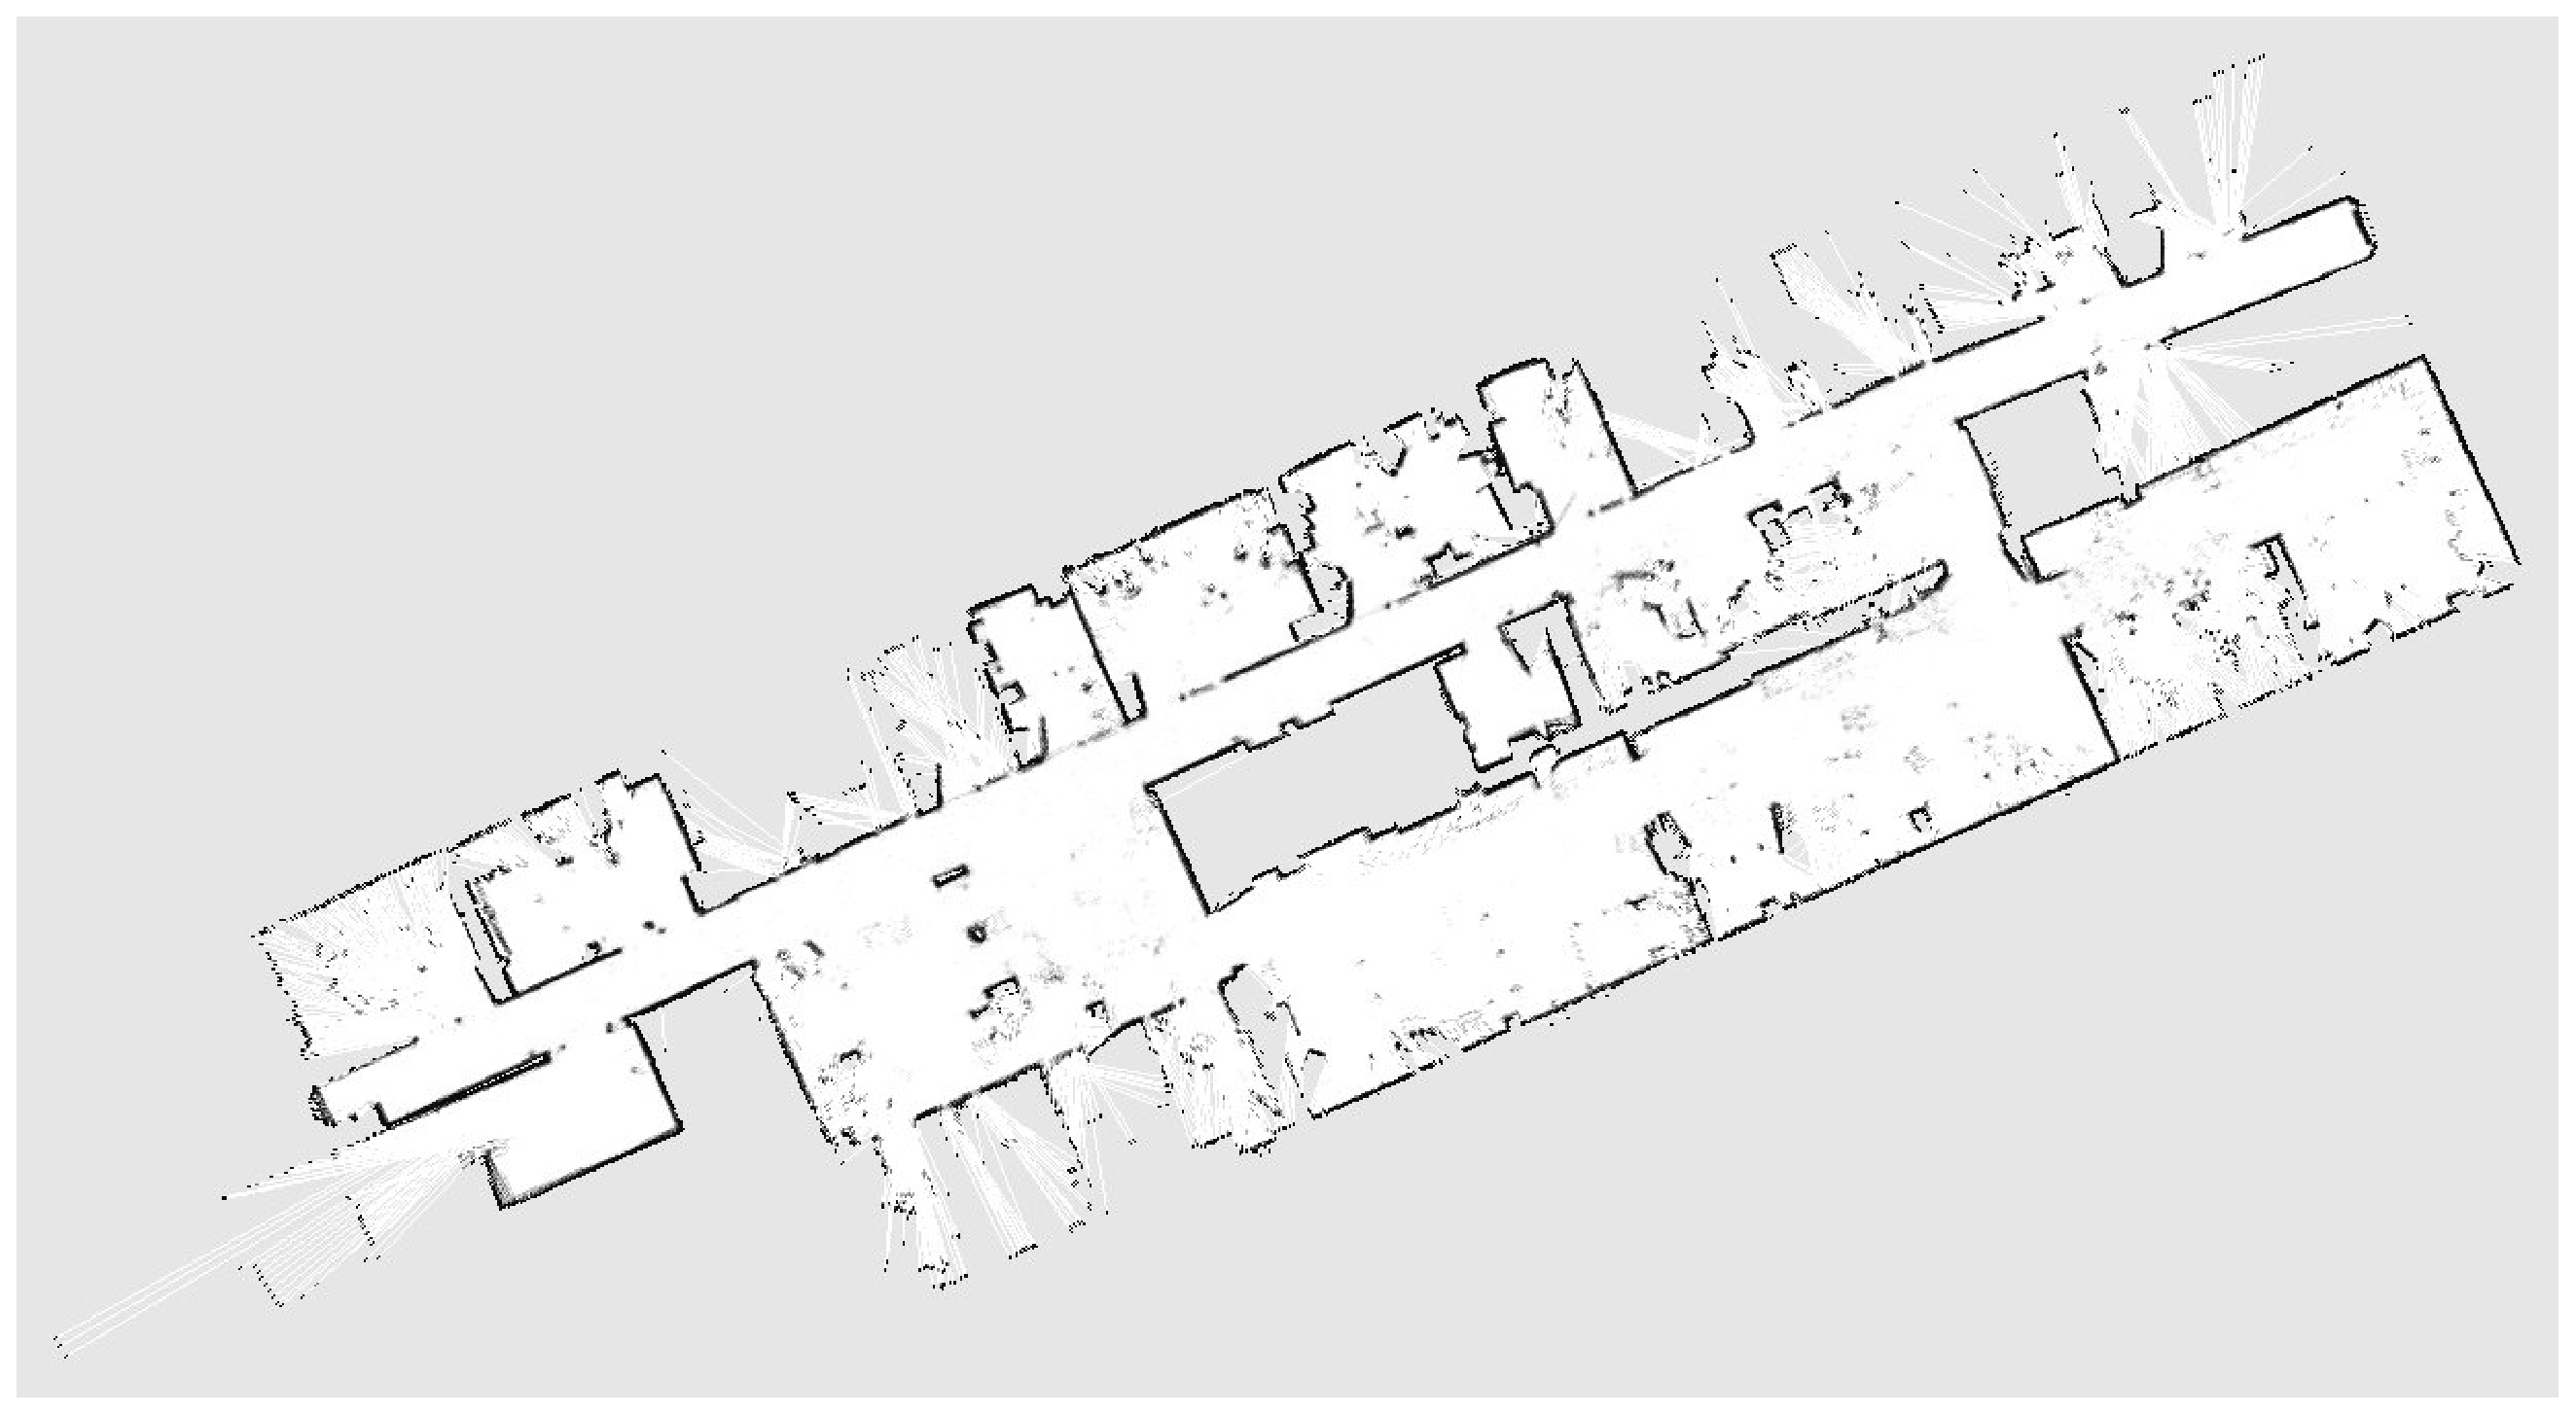
\includegraphics[width=0.45\columnwidth,keepaspectratio]{cartesium.eps}
 \label{fig:cartesium_map}
 }
 \subfigure[Freiburg, Building 079.] {
 \centering
 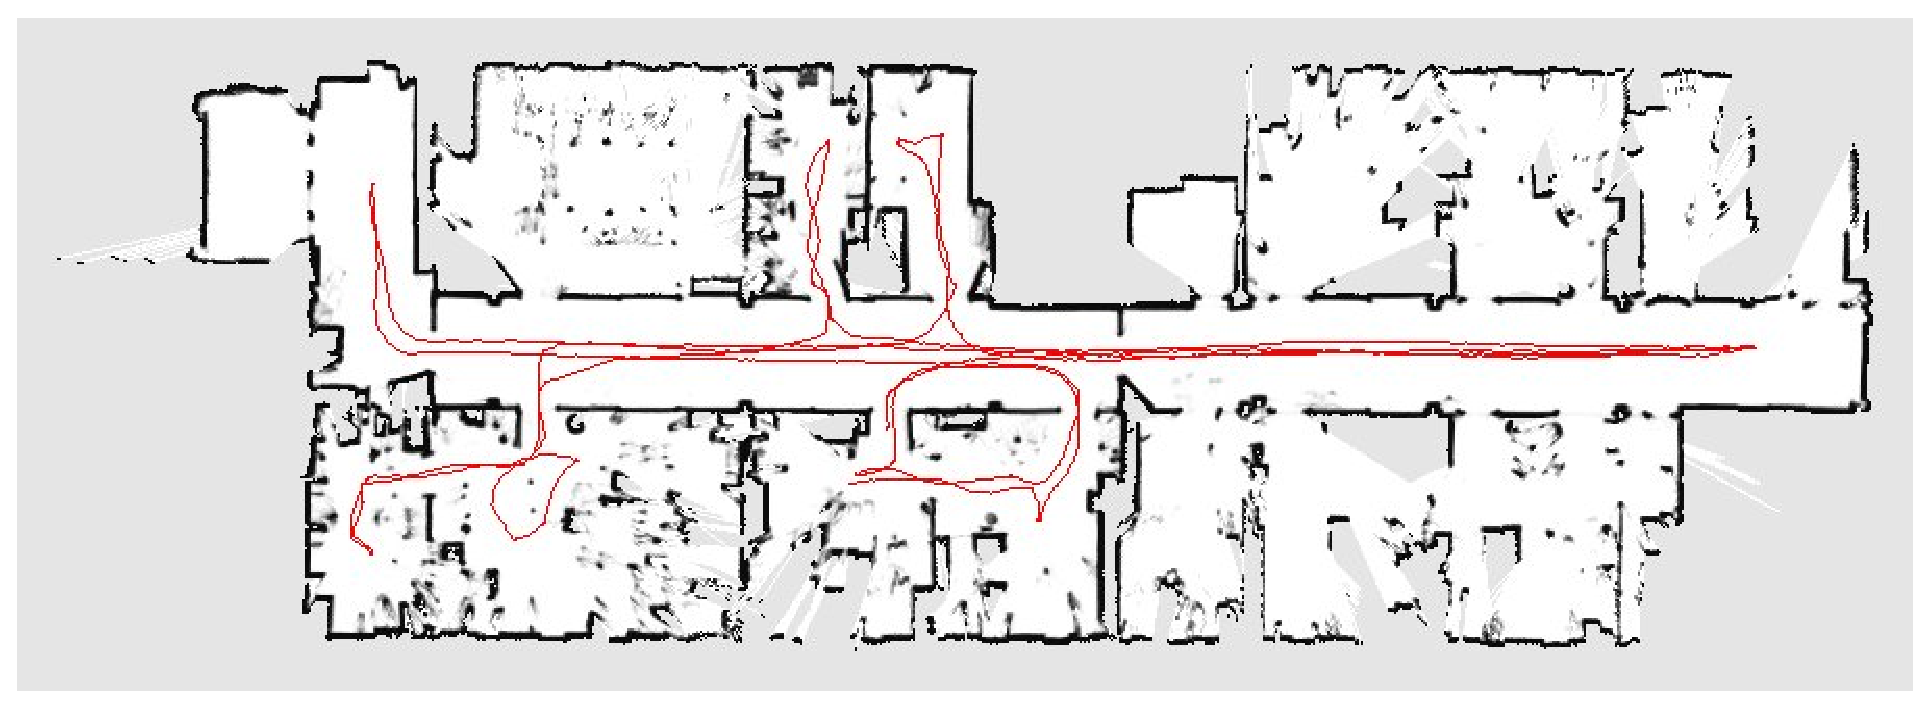
\includegraphics[width=0.45\columnwidth,keepaspectratio]{freiburg.eps}
 \label{fig:freiburg_map}
 }
 \subfigure[Outdoor dataset recorded at the University of Freiburg] {
 \centering
 
\includegraphics[width=0.45\columnwidth,keepaspectratio]{fr_campus_100p_10cm.eps}
 \label{fig:fr_campus}
 }
 \subfigure[3rd Floor of MIT CSAIL] {
 \centering
 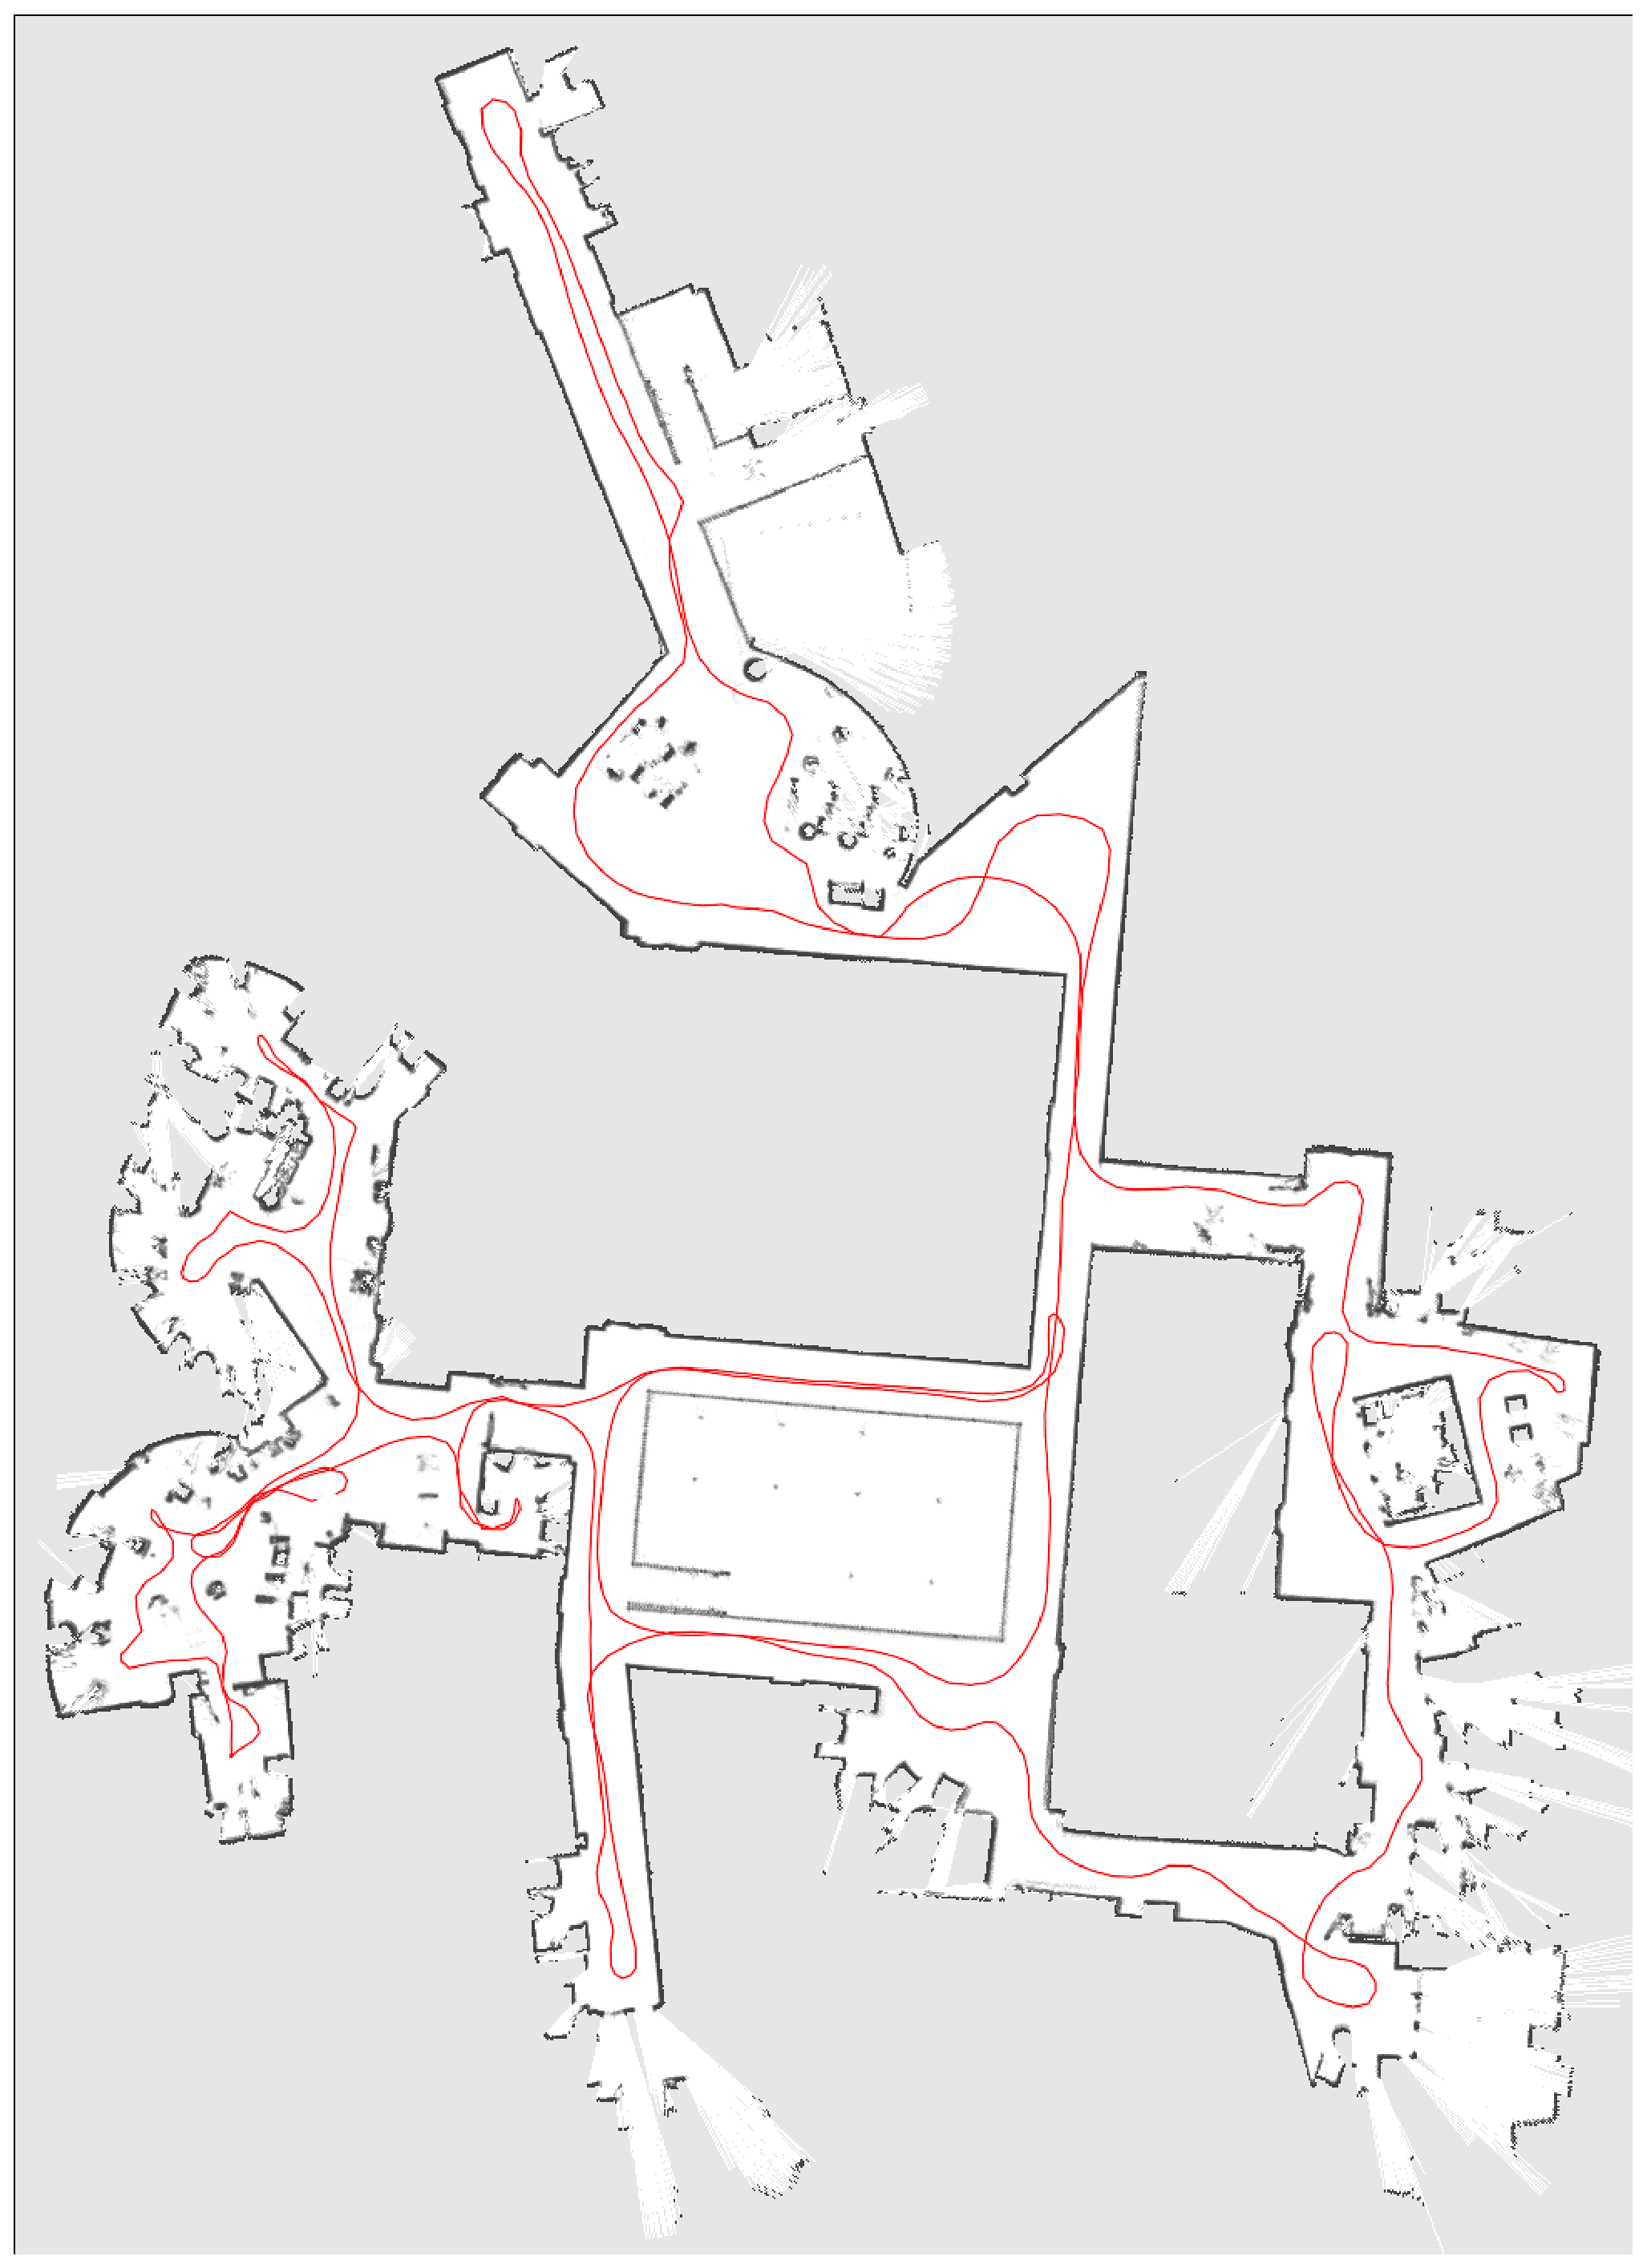
\includegraphics[angle=90,width=0.45\columnwidth,keepaspectratio]{mit-cscail-3rd-floor-2005-12-17-run4.eps}
 %\label{fig:freiburg_map}
 }
 \subfigure[Edmonton Convention Centre (site of the AAAI 2002 Grand
  Challenge)] {
 \centering
 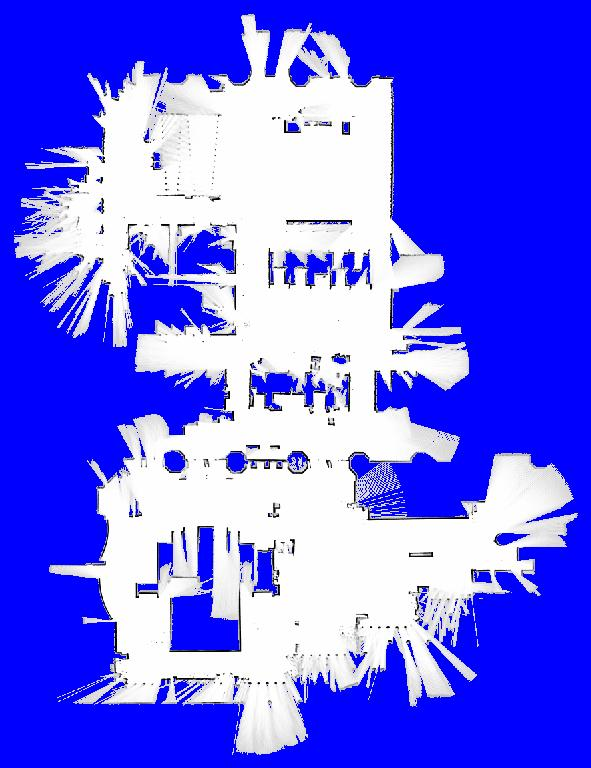
\includegraphics[angle=90,width=0.45\columnwidth,keepaspectratio]{edmonton.jpg}
 \label{fig:edmonton_center}
 }
 \caption{Testing environments.}
 \label{fig:testing_environments}
 
\end{figure}

Note that we use the exploration data (raw sensor readings and odometry) from
these data sets, and thus all algorithms use exactly the same data, form the
same robot trajectories. Thus the movement of the robot is identical, and the
only thing we examine is how quickly it can compute frontiers.

\subsection{Comparing \SOTA, \FFD, \WFD, \WFDINC and \WFDIP}
\label{section:experiments_overall_compare}
 \begin{comment}We used a desktop computer containing Intel Core 2 Duo T6600
CPU with clock speed of 2.20 GHz and Random Access Memory (RAM) in size of 4
GB.\end{comment}
%\begin{comment}
We begin by examining overall performance. We examined the run-time of all
algorithms on two different machines:
\begin{itemize}
  \item First experiment: we used a fast desktop computer containing
  Intel Core 2 Duo T6600 CPU with clock speed of 2.20 GHz, Random Access
  Memory (RAM) in size of 4 GB, L1 cache in size of 64KB (8-way Set-associative)
  and L2 cache in size of 2048KB (8-way Set-associative).
% Figure \ref{fig:graph_results_core2} shows the results of this scenario.
\item Second experiment: we used a slower desktop computer containing
Intel Pentium III (Coppermine) with clock speed of 800 MHz, Random Access
Memory (RAM) in size of 1 GB, L1 cache in size of 32KB (4-way Set-associative)
  and L2 cache in size of 256KB (4-way Set-associative). Research-grade robots
  typically have a faster CPU, but commercial robots typically do not.
 % Figure \ref{fig:graph_results_coppermine} shows the results of this scenario.
\end{itemize} 
%\end{comment}


\FFD is called every-time a new laser reading is received. Therefore, in
order to compare \FFD execution time to other algorithms correctly, we
accumulate \emph{FFD}'s execution times between calls to other algorithms. In
other words, if we call \WFD in time-stamps $t_i$ and $t_{i+1}$, then
\emph{FFD}'s accumulated execution time is calculated by: 

\begin{displaymath}
\sum_{x = t_i}^{t_{i+1}}{ExecutionTime_{FFD}(x)}
\end{displaymath}

Moreover, we remind the reader that because \FFD is called for every particle
in the particle-filtering GMapping~\cite{grisetti07tro},
the results here accumulate also over the number of particles (30 in our case).

Figure \ref{fig:graph_results} shows
%one set of
results of the comparison in each of the two machines. Each
group of bars represents a run over a separate map. For each algorithm, we
calculate the mean execution time, over the duration of the exploration. The vertical axis
measures the calculated execution time in microseconds, on a \emph{logarithmic scale}.
%XXX Tell us what we see:
The one-second line is at $10^6$ microseconds. The next tick, at $10^7$, marks
10 seconds.

Figure \ref{fig:graph_results} shows that \WFD is faster than \SOTA
by approximately one order of magnitude. \FFD is faster than \WFD by
one to two orders of magnitude. Indeed, \FFD performs close to the one-second
line.  In contrast, \WFD and \SOTA typically take anywhere from 10 to 100 seconds
to perform their task, even on relatively fast machines. Surprisingly, we
discovered that \WFDIP often performs frontier detection in the shortest
execution time. The reason is that \WFDIP contains a well balance between the
frequency of number of calls (only on \mapevent s). On the one hand, \WFD
algorithm has to detect all frontiers in each execution because it does not
utilize previous detected frontiers. On the other hand, \FFD algorithm keeps
utilizing previous detected frontiers but in price of keep running the
maintenance routine in the background. \WFDIP algorithm is an hybrid approach
that reduces the number of calls (relatively to \FFD) while performing frontier
detection on a smaller search domain (relatively to \WFD).

\begin{figure} 
 \centering
 \subfigure[Intel T6600] {
	 \centering
	%  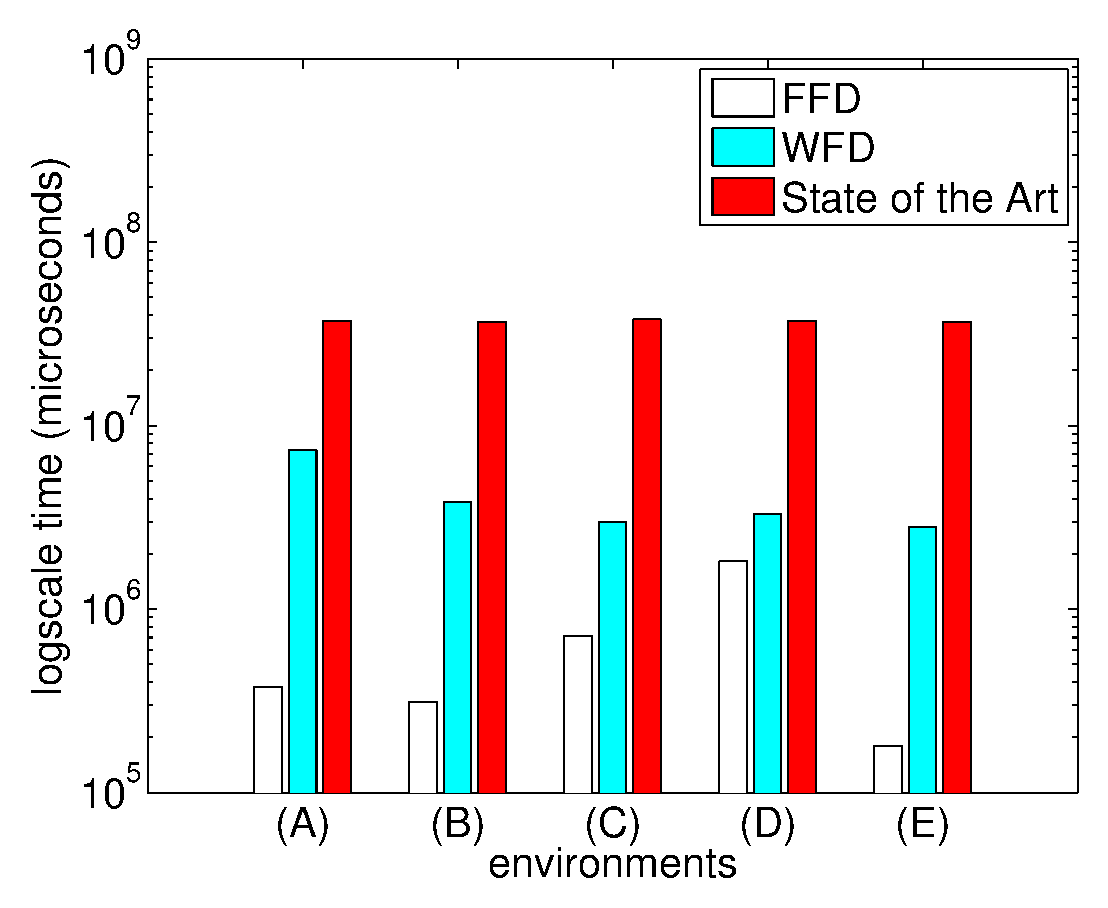
\includegraphics[width=0.8\columnwidth,keepaspectratio,angle=0]{graphs/graph_Results_core2.eps}
	 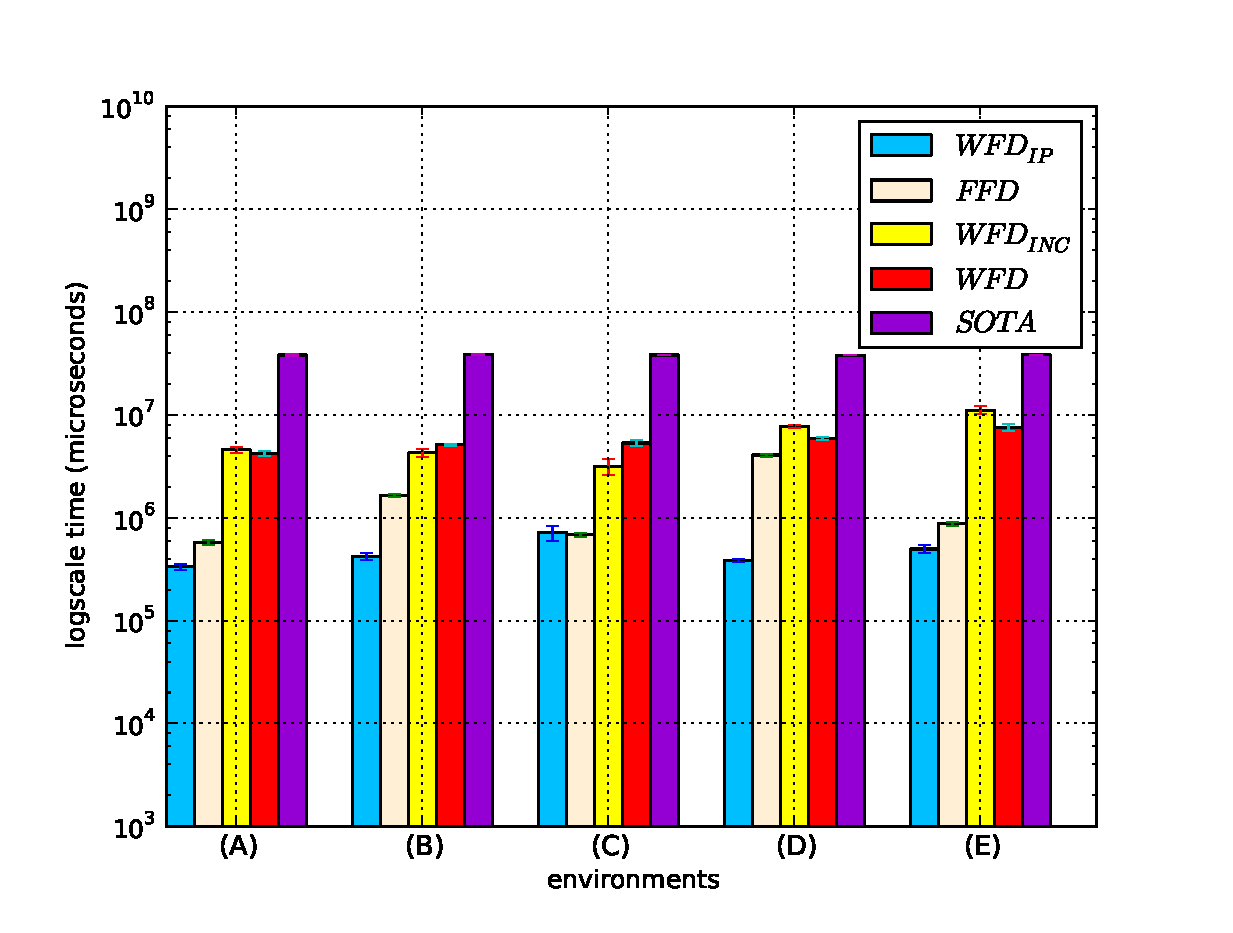
\includegraphics[width=0.8\textwidth,keepaspectratio,angle=0]{plot_Results_five_algorithms.eps}
	 \label{fig:graph_results_core2}
 } 
 \subfigure[Intel Coppermine] {
 \centering
 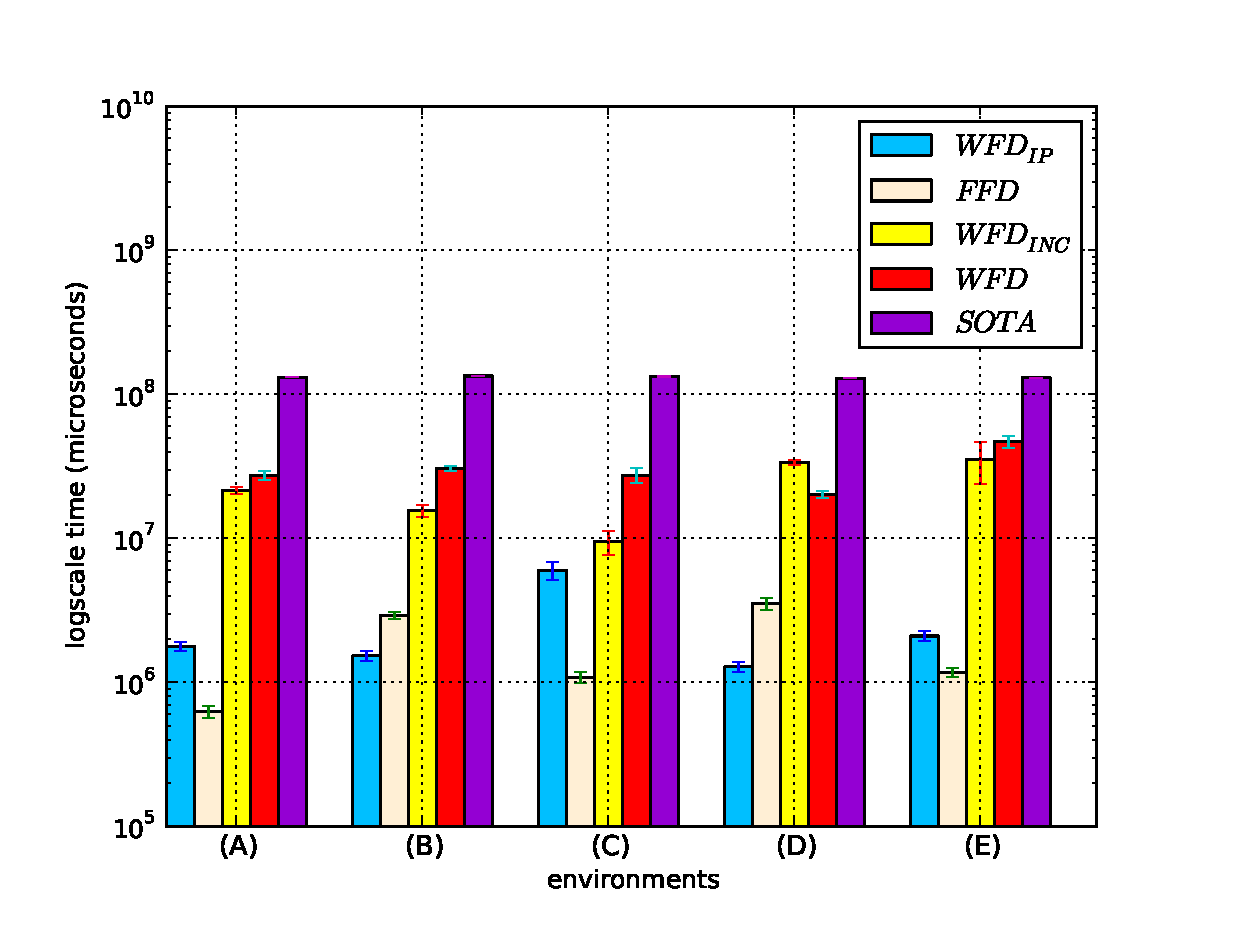
\includegraphics[width=0.8\columnwidth,keepaspectratio,angle=0]{plot_Results_coppermine.eps}
 \label{fig:graph_results_coppermine}}
 
 \caption{Comparing all versions of \WFD and \FFD to State-of-the-Art algorithm
 on different machines.}
 \label{fig:graph_results}
\end{figure}

\emph{FFD}'s improvement over \SOTA and \WFD is indeed notable, given that
the measured results are not for single \FFD runs, but in fact show
accumulated run-time, over the frequency of the sensor readings, multiplied
over the number of particles (approximately 2000 calls to \FFD for each \WFD or \SOTA calls).
These multiplicative factors have significant impact on \emph{FFD}'s usability. 
It is important to understand whether the number of particles influences the result
more than the frequency of sensor readings, as the number of particles
is often increased for better quality. We discuss this in detail in Section
\ref{section:experiments_ffd_finer_resolution}.

\subsubsection{What Happened in Environment (D)?}
If we take a closer look at the results shown in Figure \ref{fig:graph_results_core2},
in environment (D) the mean run-time of \WFD is relatively not much slower than
\FFD. Environment (D) contains plenty of regions that seems to have small
obstacles which enlarge the length of the contour scanned by \FFD. In Section
\ref{section:ffd_complexity} we showed an upper bound of \FFD's run-time
complexity (Equation \eqref{eq:ffd_complexity_with_freq}). One of the factors
that affect the boundary is the contour length that is scanned by \FFD algorithm
(Section \ref{section:detecting_new_frontiers}). Figure
\ref{fig:ffd_worst_case_contour} shows an example of the enlargement of the
contour when the robot arrives to a crowded region. Thus, The empirical results
shown in this section well-support the theoretical boundary.

\begin{figure} 
 \centering
 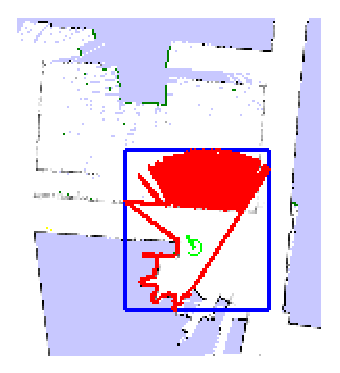
\includegraphics[width=0.4\columnwidth,keepaspectratio,angle=0]
 {images/environment_D_bad_contour_example2.eps}
 \caption{An example of \FFD's worst-case as shown in Environment (D)}
 \label{fig:ffd_worst_case_contour}
\end{figure}

\subsubsection{Why is \WFDINC Sometimes Worse than \WFD?}
In the worst-case, \WFDINC algorithm should perform the
same as \WFD including an overhead of maintenance. However, 
as can be seen in Figure \ref{fig:graph_results}, the run-time means of
\WFD and \WFDINC do not have a specific trend.

We hypothesize that in certain environments, where there is a high frequency
of active particle change, \WFDINC cleans its previous detected frontiers
more often, and this explains its run-time.

We provide evidence to support this hypothesis in Table
\ref{table:active_particle_changes} and Figure
\ref{fig:graph_active_particle_changes}.
Table \ref{table:active_particle_changes} shows the particle changes in
different environments. Each row represents a single environment. The first column contains the environment identifier. The second column contains the
number of active particle changes. The third column contains the total number
of executions and the forth column contains the percentage of particle
changes relative to the total number of executions. 

Figure \ref{fig:graph_active_particle_changes} shows the active particle changes
over time. For a specific environment, the vertical axis represents each execution
and the horizontal axis represents whether the active particle was changed
(\emph{Yes} for a change and \emph{No} otherwise). There is an exception in
environment (C) in which the active particle changes percent is quite low but
\WFDINC's execution time is still worse than \WFD's execution time. Here, the
explored environment is very large and hence, for each change, the robot
has to detect frontiers in a very large area, in contrast to other environments.
\begin{table}
\centering
\begin{tabular}{|c|c|c||c|}
\hline \textbf{Map}&\textbf{Changes}&\textbf{Executions}&\textbf{Percent (\%)}
\\
\hline 
\hline (A)& 56 & 110 & 50.91  \\
\hline (B)& 52 & 287 & 18.12  \\
\hline (C)& 25 & 160 & 15.62  \\
\hline (D)& 193 & 429 & 44.99 \\ 
\hline (E)& 73 & 340 & 21.47 \\ \hline
\end{tabular}
\caption{Comparing active particle changes in different environments.}
\label{table:active_particle_changes}
\end{table}

\begin{figure}[htp]
% XXX Matan, print out a copy of the paper, and check whether the labels are legible. I can barely read
% them on my screen, even if I zoom. But perhaps it's just my screen.  If they are not legible, you need
% to enlarge the fonts on the labels.
 \centering 
 \subfigure[Cartesium Building, Bremen] {
 \centering
 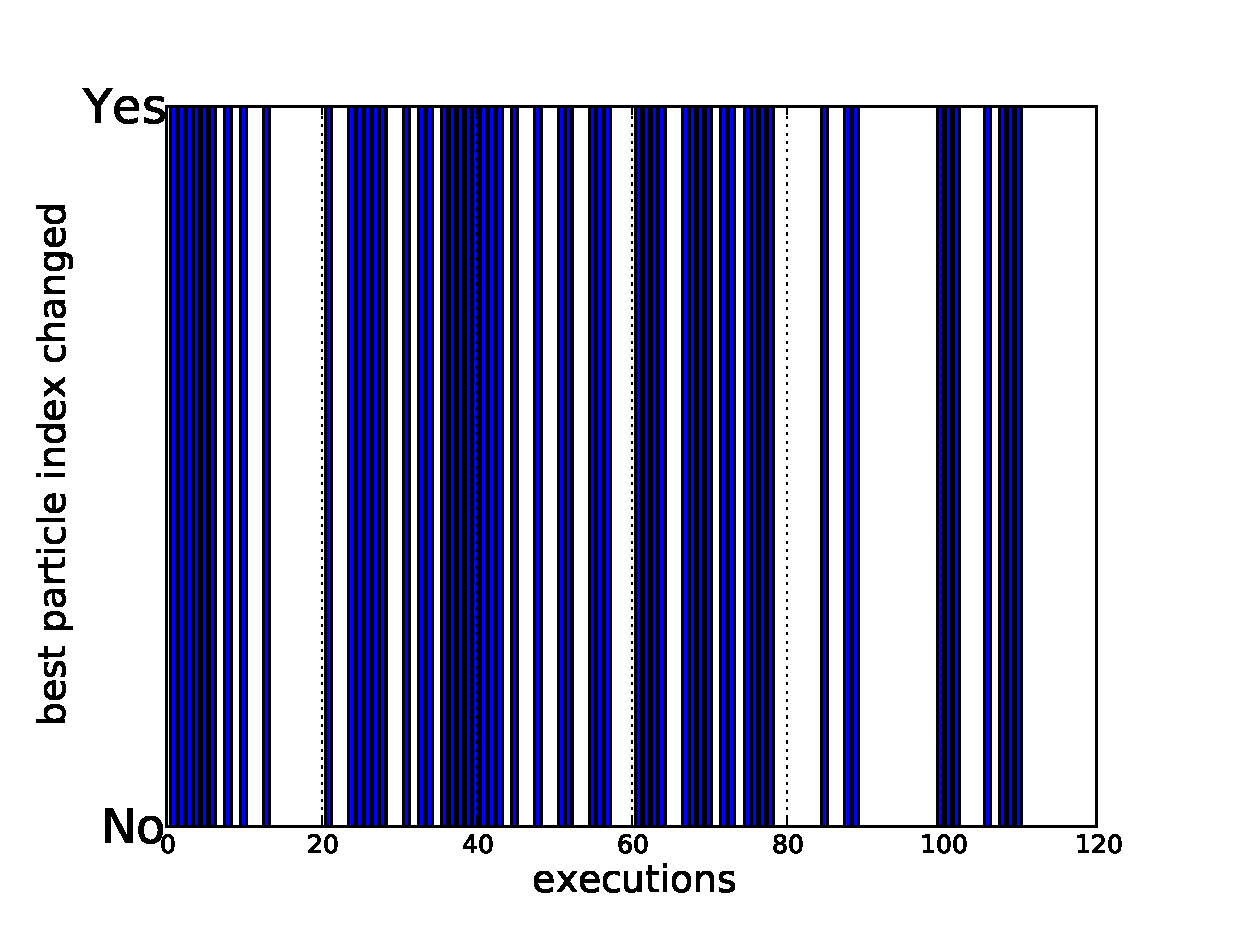
\includegraphics[width=0.45\columnwidth,keepaspectratio]{plot_best_particle_index_ubremen-cartesium-demo2.eps}
 } 
 \subfigure[Freiburg, Building 079] {
 \centering
 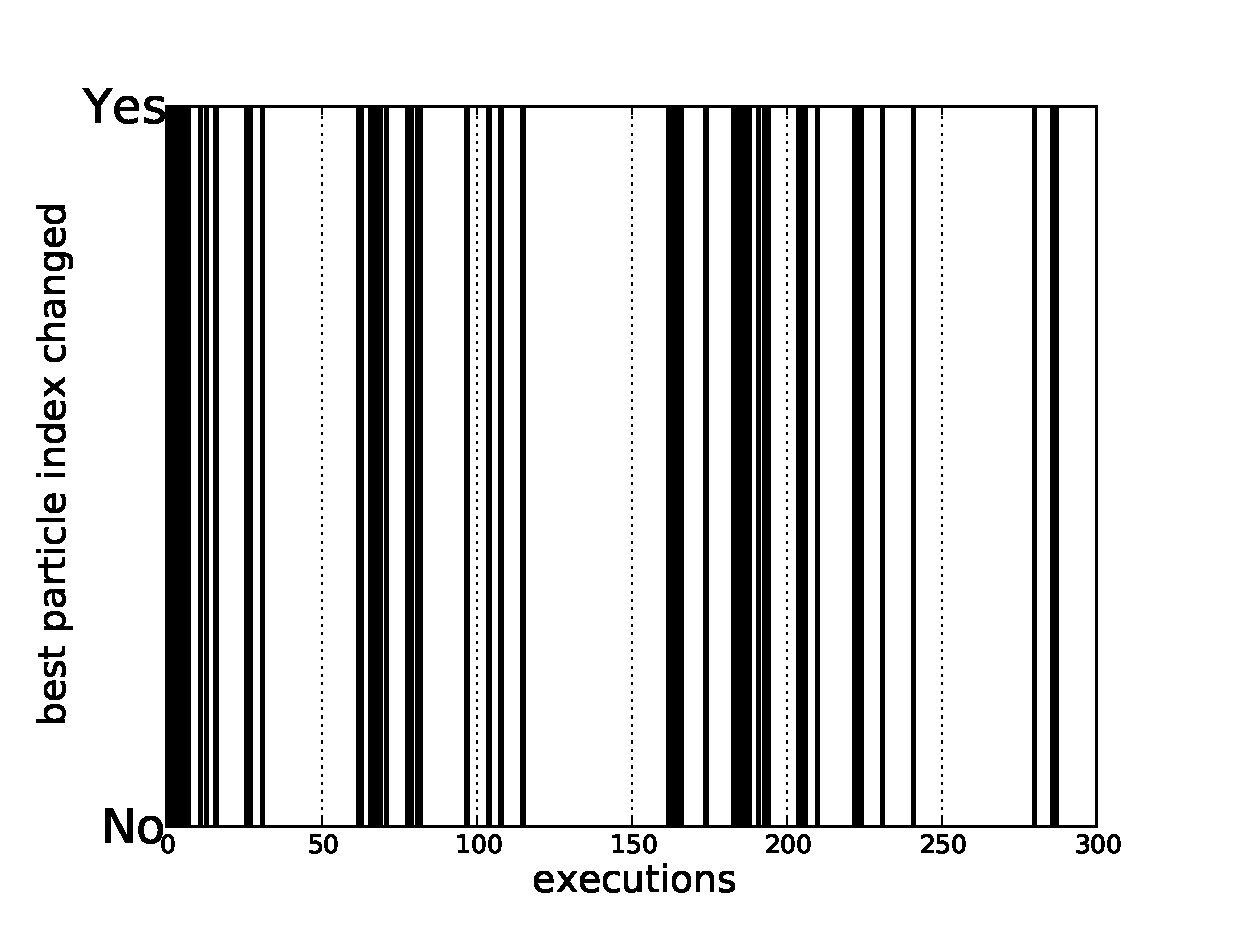
\includegraphics[width=0.45\columnwidth,keepaspectratio]{plot_best_particle_index_fr079-sm.eps}
 }
 \subfigure[Outdoor dataset, University of Freiburg] {
 \centering
 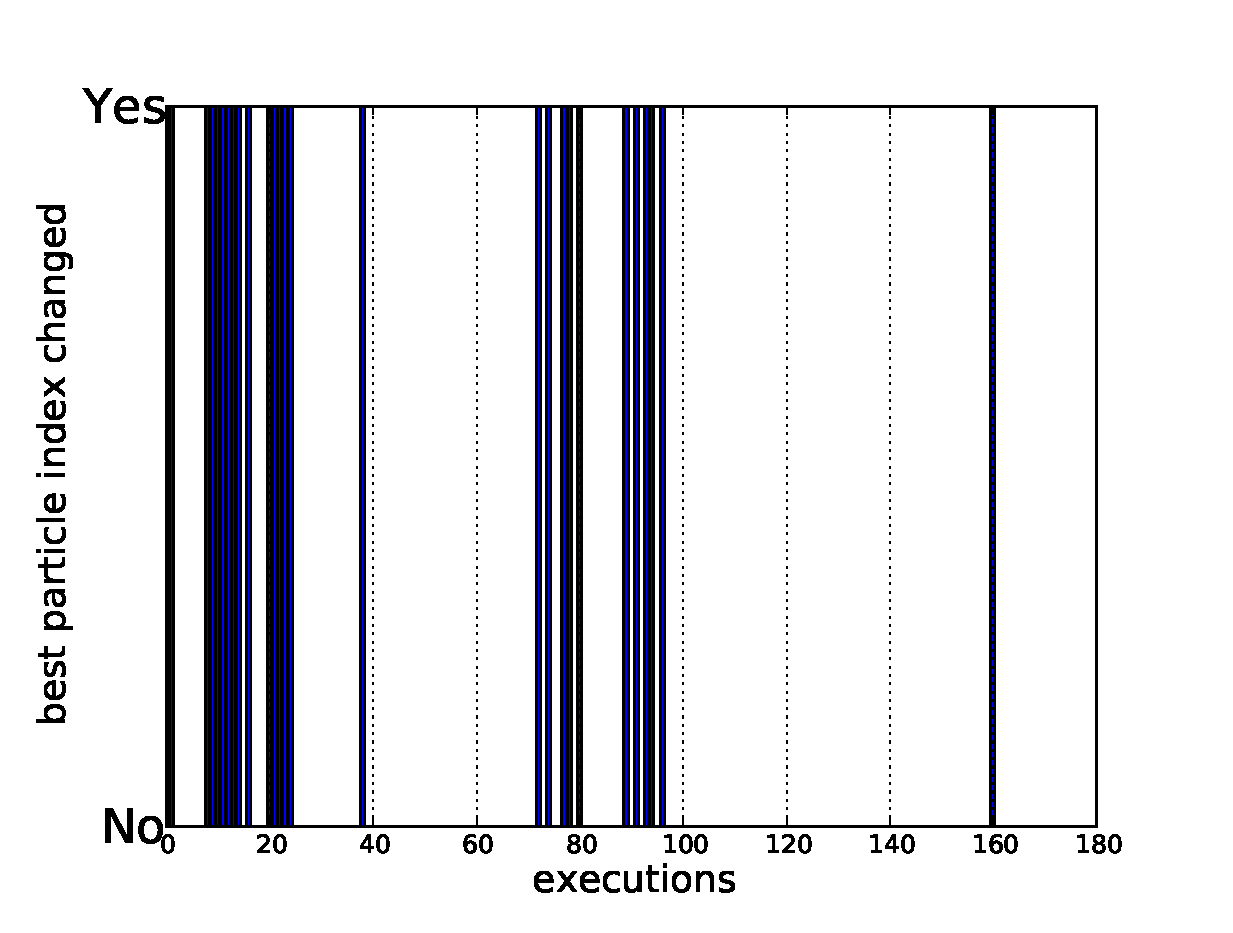
\includegraphics[width=0.45\columnwidth,keepaspectratio]{plot_best_particle_index_fr-campus-20040714.eps}
 }
 \subfigure[3rd Floor of MIT CSAIL] {
 \centering
 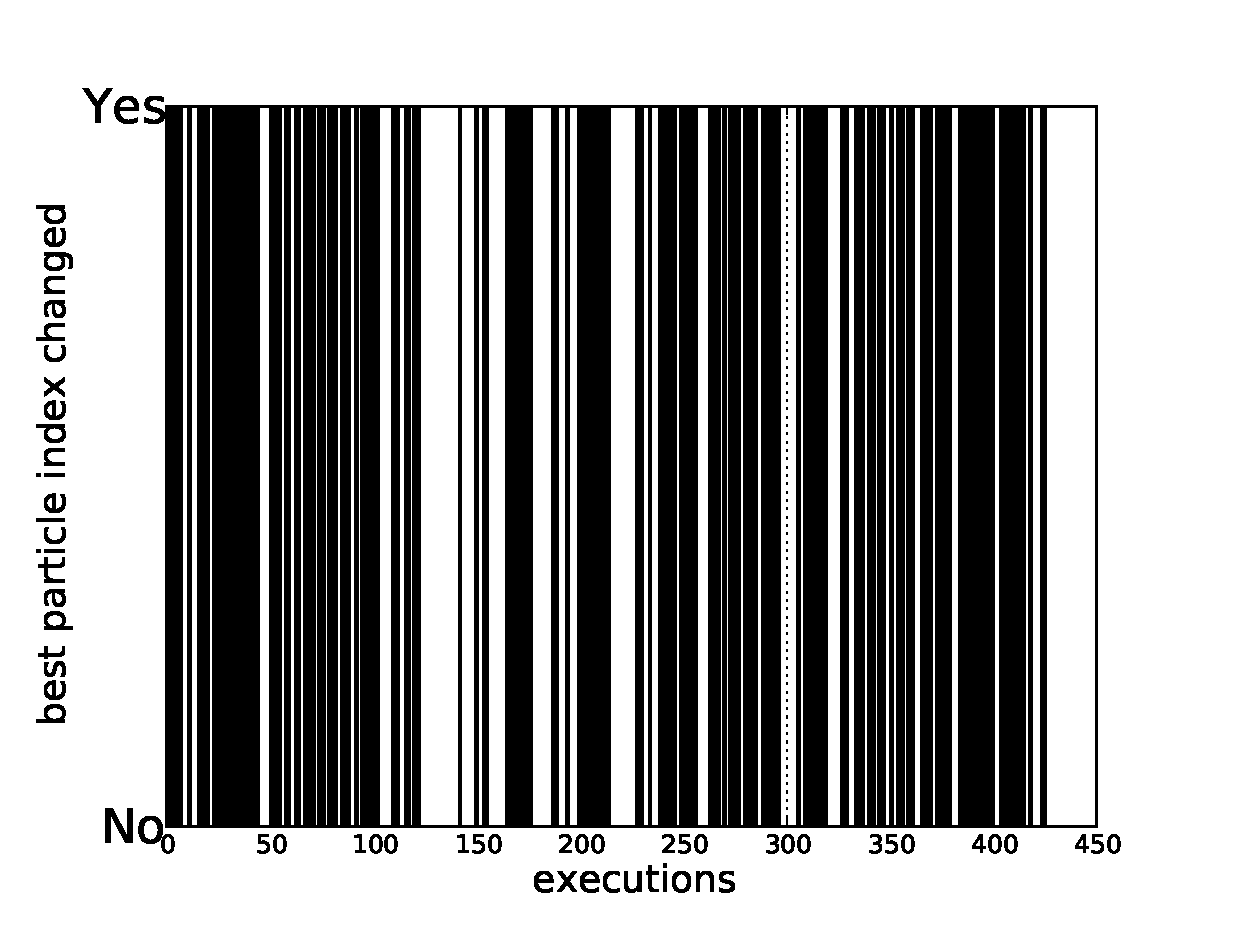
\includegraphics[width=0.45\columnwidth,keepaspectratio]{plot_best_particle_index_mit-csail-3rd-floor-2005-12-17-run4.eps}
 }
 \subfigure[Edmonton Convention Centre] {
 \centering
 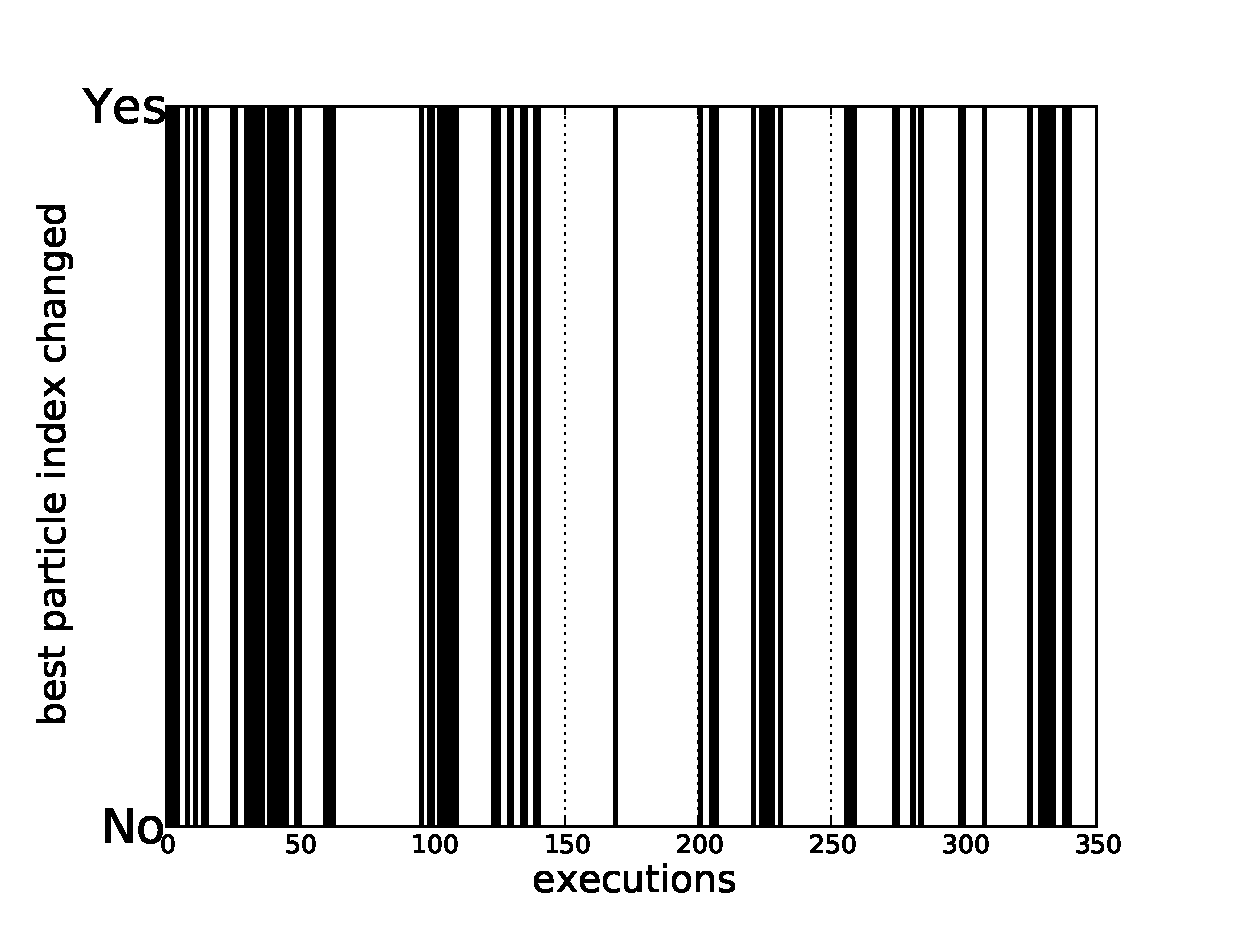
\includegraphics[width=0.45\columnwidth,keepaspectratio]{plot_best_particle_index_edmonton_3.eps}
 }
 \caption{Changes in Active Particle Over Executions.}
 \label{fig:graph_active_particle_changes}
\end{figure}

\subsubsection{What Happened to \WFDIP in Environments (A),(C),(E), Figure
\ref{fig:graph_results_coppermine}?}
\label{section:what_happend_to_wfdip_on_weak_machine}
Figure \ref{fig:graph_results} shows the run-time results of all algorithms on
two testing machines. On the stronger machine (Figure~\ref{fig:graph_results_core2}) \WFDIP outperforms all other algorithms. However,
on the weaker machine (Figure \ref{fig:graph_results_coppermine}), the situation
is different in environments (A),(C) and (E). 

The two machines differ in both memory size and number of cores.
The Coppermine machine is equipped with less random access memory (1 GB) than
the stronger machine (4 GB). The key feature of \WFDIP is
its robustness against changes in active particle since it holds a separate
instance of \WFDINC for each particle. In our implementation, there
are 30 particles and hence, \WFDIP holds 30 instances of \WFDINC (i.e., 30
frontier databases, 30 maps etc. ). In addition, the Coppermine machine is
equipped with a single core CPU, in contrast to the stronger machine that is
equipped with 2 cores. The GMapping SLAM system runs two threads (a \emph{main} thread
and a \emph{SLAM} thread). We believe that the stronger machine allows each thread to run on a separate core.

There thus remains a question as to the reason for such behavior of \WFDIP relates to either the 
lack of memory or to the single core of the weaker machine. To determine this,
we bounded the memory of the strong machine to be 1GB. The behavior of \WFDIP remained 
the same (we forgo adding the redundant figure here). The conclusion is therefore that
the number of cores caused the differences in \WFDIP's behavior. This should
be taken into account when choosing between \FFD and \WFDIP for a given robot CPU.

\subsection{Evaluating \FFD at a Finer Resolution}
\label{section:experiments_ffd_finer_resolution}
We turn to evaluating \FFD more closely.
Figure \ref{fig:graph_particle_times} compares the run-time of individual particles
in specific environments. Each bar represents a specific particle. The vertical axis measures the
mean run-time of \FFD for the particle. The
error-bars represent the standard deviation of each particle's run-time. 

The figure shows that the per-particle run-time is measured in a few hundred micro-seconds.
Thus the overall results were accumulating comparing the accumulation of thousands
of \FFD runs against single \WFD and \SOTA runs.  Indeed, one can boost \FFD's execution time by not executing it on 
every received laser reading, since the frequency of receiving new laser readings is often 
higher than the speed of processing and updating the map anyways.  Many laser sensors
generate output at 30Hz--75Hz, at least three times faster than the rate at which the robots
process the information.  By ignoring some laser readings, \FFD would perform much better, without
any noticeable decay in mapping quality.

% \begin{figure}
%  \centering
%  \includegraphics[width=0.9\columnwidth,keepaspectratio]{images/graph_Results.\image_ext}
%  \caption{Comparing WFD and FFD to State-of-the-Art algorithm.}
%  \label{fig:graph_results_core2}
% \end{figure}




\begin{figure}[htp]
% XXX Matan, print out a copy of the paper, and check whether the labels are legible. I can barely read
% them on my screen, even if I zoom. But perhaps it's just my screen.  If they are not legible, you need
% to enlarge the fonts on the labels.
 \centering 
 \subfigure[Cartesium Building, Bremen] {
 \centering
 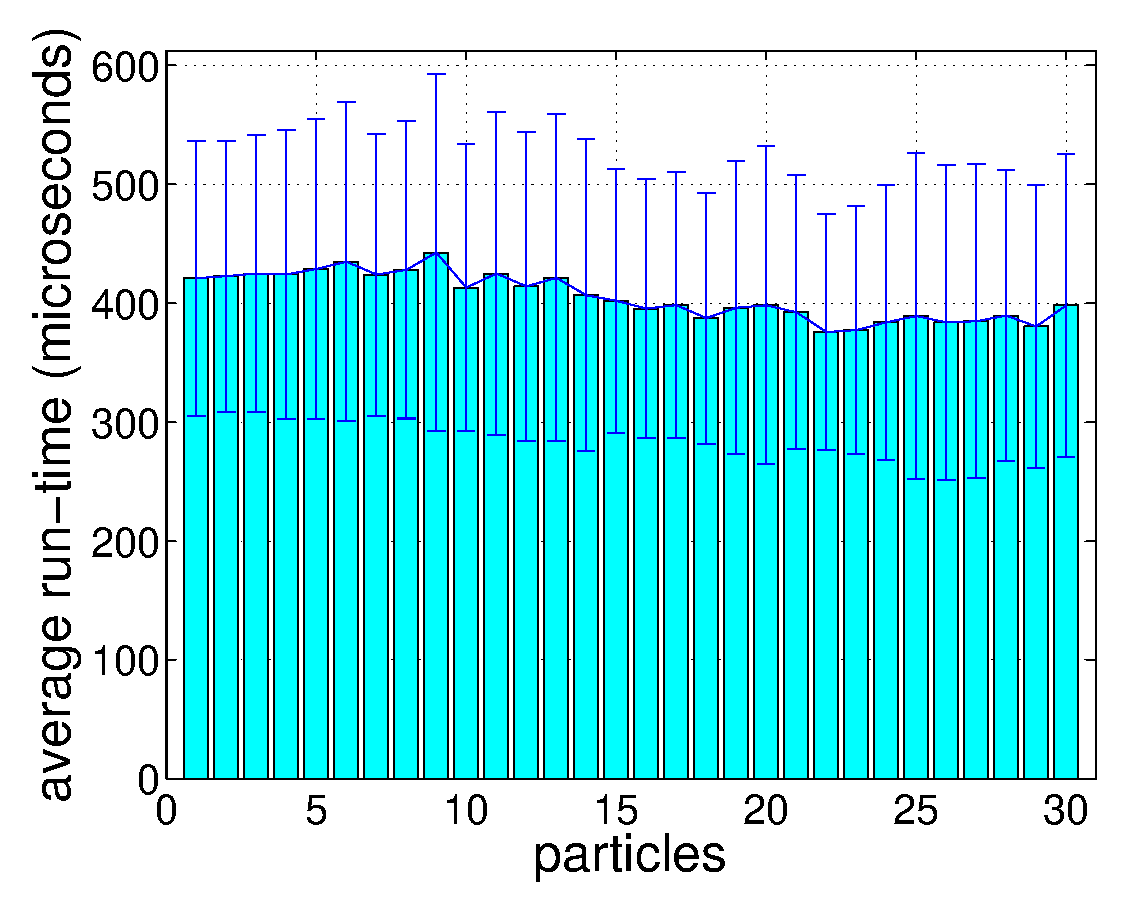
\includegraphics[width=0.45\columnwidth,keepaspectratio]{graph_particle_times_ubremen-cartesium-demo2.eps}
 \label{fig:graph_particle_times_cartesium}} 
 \subfigure[Freiburg, Building 079] {
 \centering
 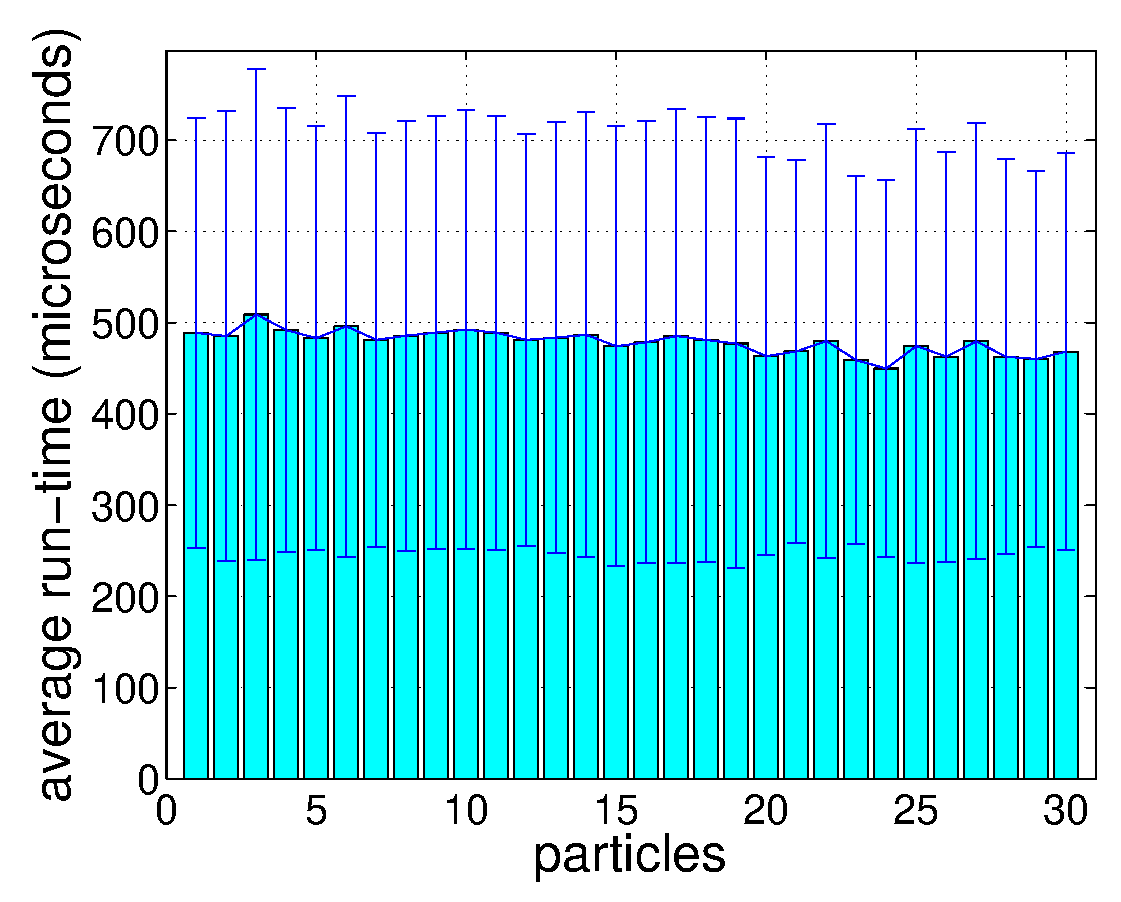
\includegraphics[width=0.45\columnwidth,keepaspectratio]{graph_particle_times_fr079-sm.eps}
 \label{fig:graph_particle_times_fr079}}
 \subfigure[Outdoor dataset, University of Freiburg] {
 \centering
 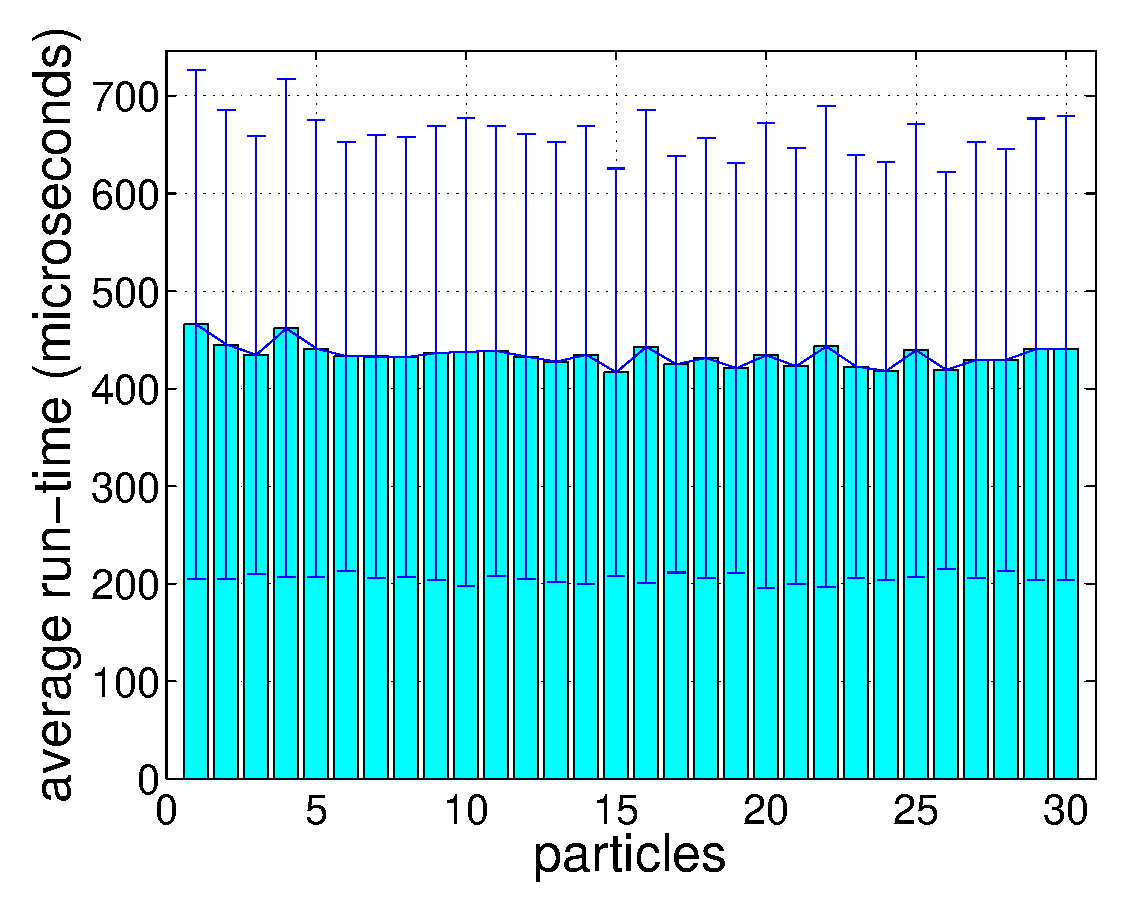
\includegraphics[width=0.45\columnwidth,keepaspectratio]{graph_particle_times_fr-campus-20040714.eps}
 \label{fig:graph_particle_times_fr_campus}}
 \subfigure[3rd Floor of MIT CSAIL] {
 \centering
 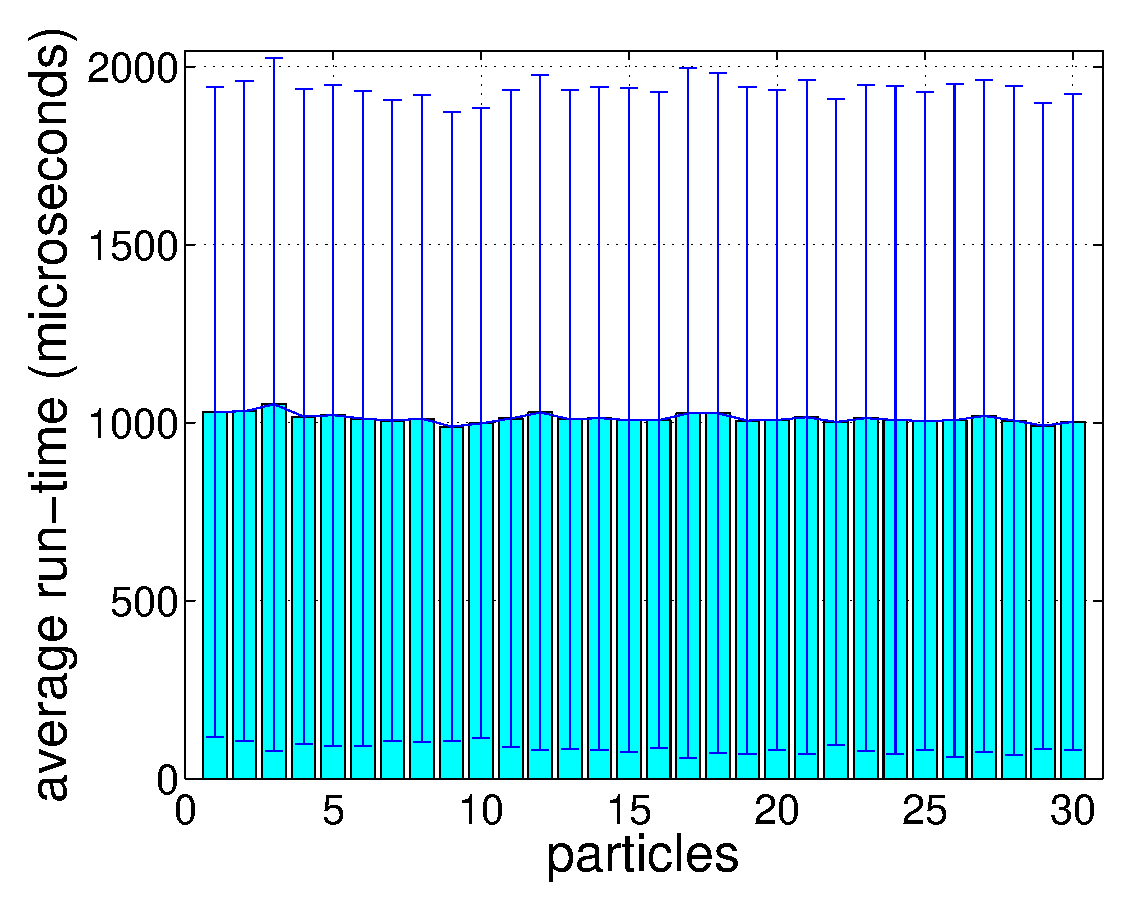
\includegraphics[width=0.45\columnwidth,keepaspectratio]{graph_particle_times_mit-csail-3rd-floor-2005-12-17-run4.eps}
 \label{fig:graph_particle_times_mit-csail}}
 \subfigure[Edmonton Convention Centre] {
 \centering
 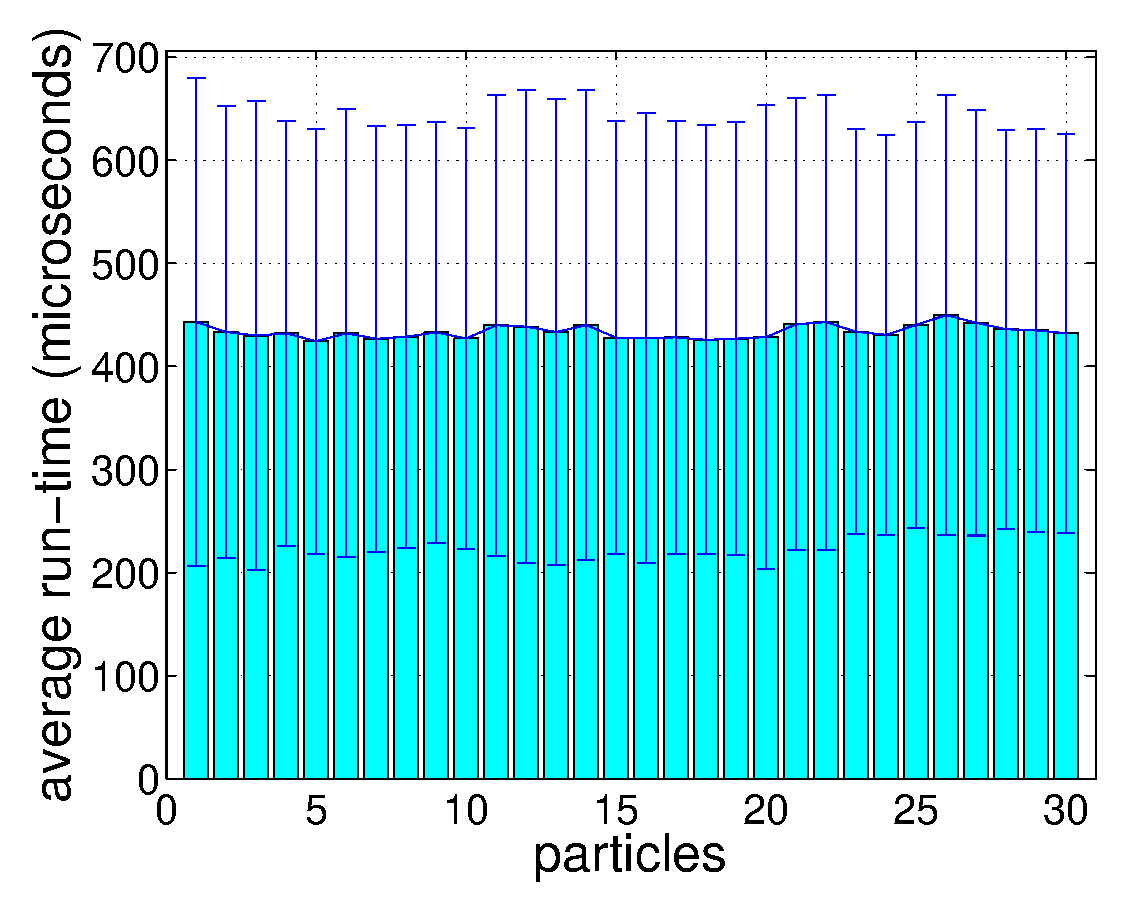
\includegraphics[width=0.45\columnwidth,keepaspectratio]{graph_particle_times_edmonton_3.eps}
 \label{fig:graph_particle_times_edmonton}}
 \caption{\FFD run-time for individual SLAM particles.}
 \label{fig:graph_particle_times}
\end{figure}

\paragraph{\FFD's Performance According to Number of Particles}
One of \FFD's drawbacks is that in order to get a complete picture of frontiers
in a given time, it has to persistently run in the background. As mentioned in
Section \ref{section:ffd_maintaining_previously_detected_frontiers}, if \FFD is
integrated into a particle-filter based SLAM implementation, each particle has
its own instance of \FFD algorithm and hence, the overall run-time is increased.
Figure \ref{fig:graph_ffd_run-time_vs_particle_numbers} compares the mean
run-time of \FFD by changing the number of particles in specific
environments.
Each bar represents a run of \FFD with a specific number of particles. The
vertical axis measures the mean run-time of \FFD for the configuration.
The error-bars represent the standard deviation of each configuration's
run-time.


\begin{figure}[htp]
 \centering 
 \subfigure[Cartesium Building, Bremen] {
 \centering
 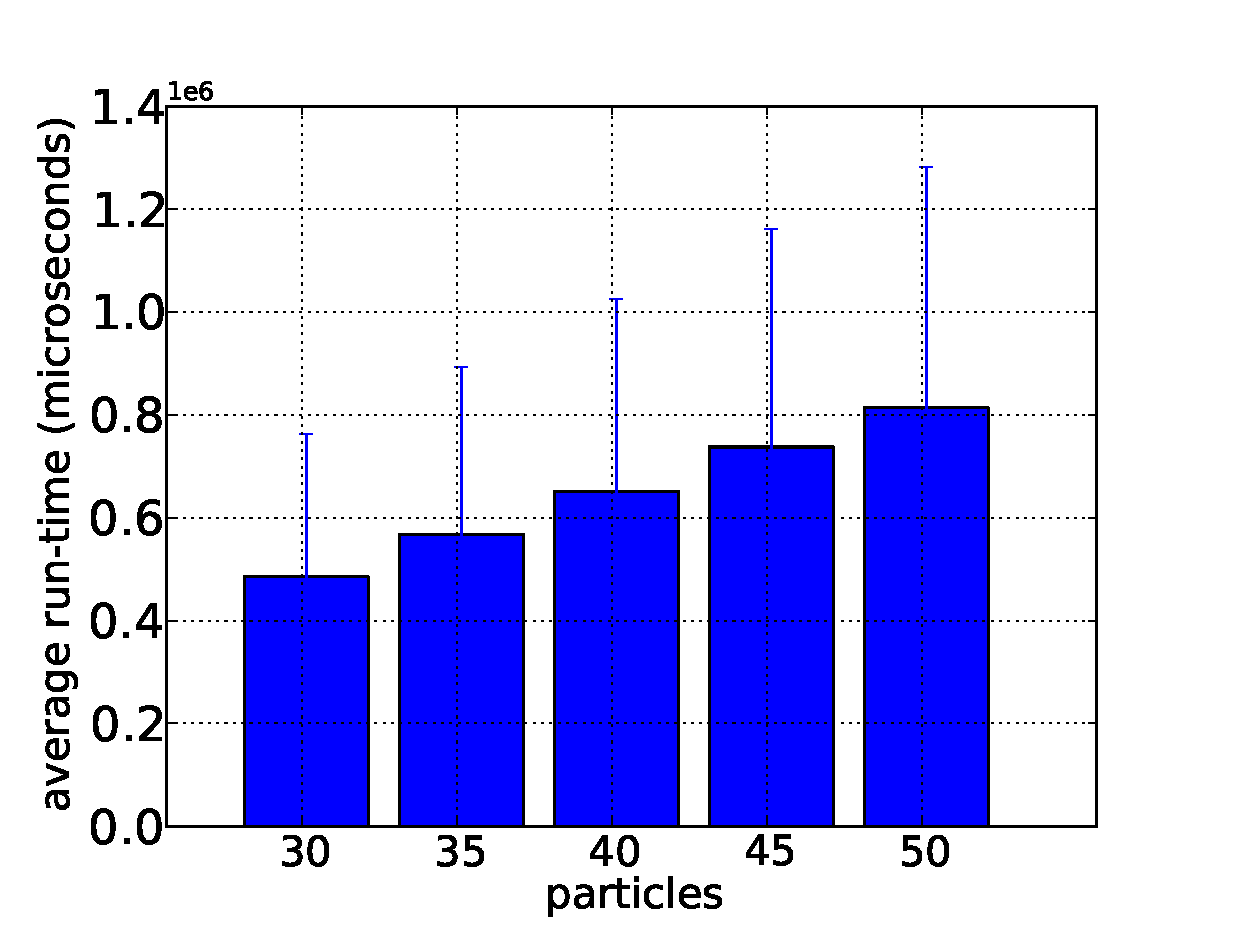
\includegraphics[width=0.45\columnwidth,keepaspectratio]{plot_ubremen-cartesium-demo2_gfs_log_Particles.eps}
 } 
 \subfigure[Freiburg, Building 079] {
 \centering
 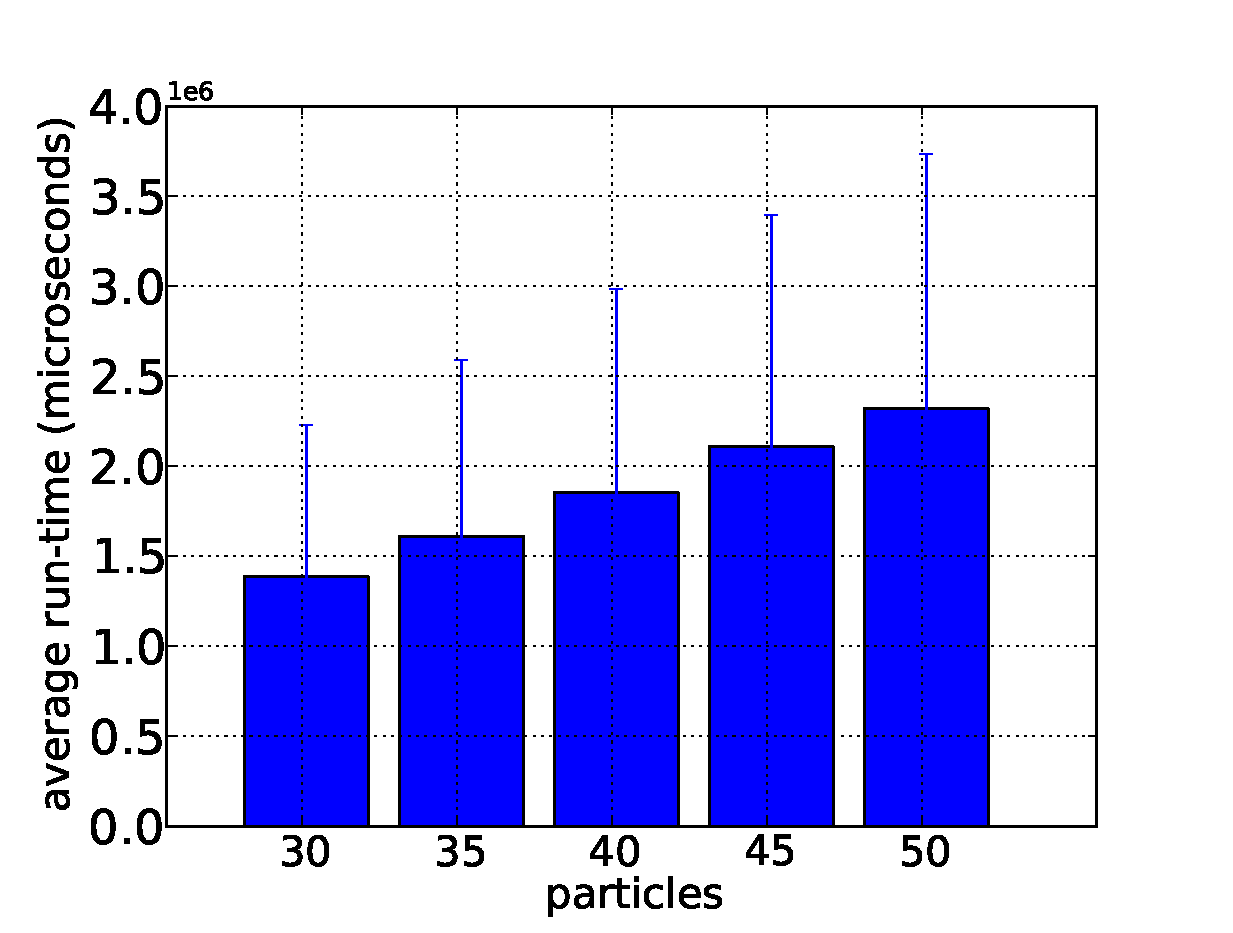
\includegraphics[width=0.45\columnwidth,keepaspectratio]{plot_fr079-sm_log_Particles.eps}
 }
 \subfigure[Outdoor dataset, University of Freiburg] {
 \centering
 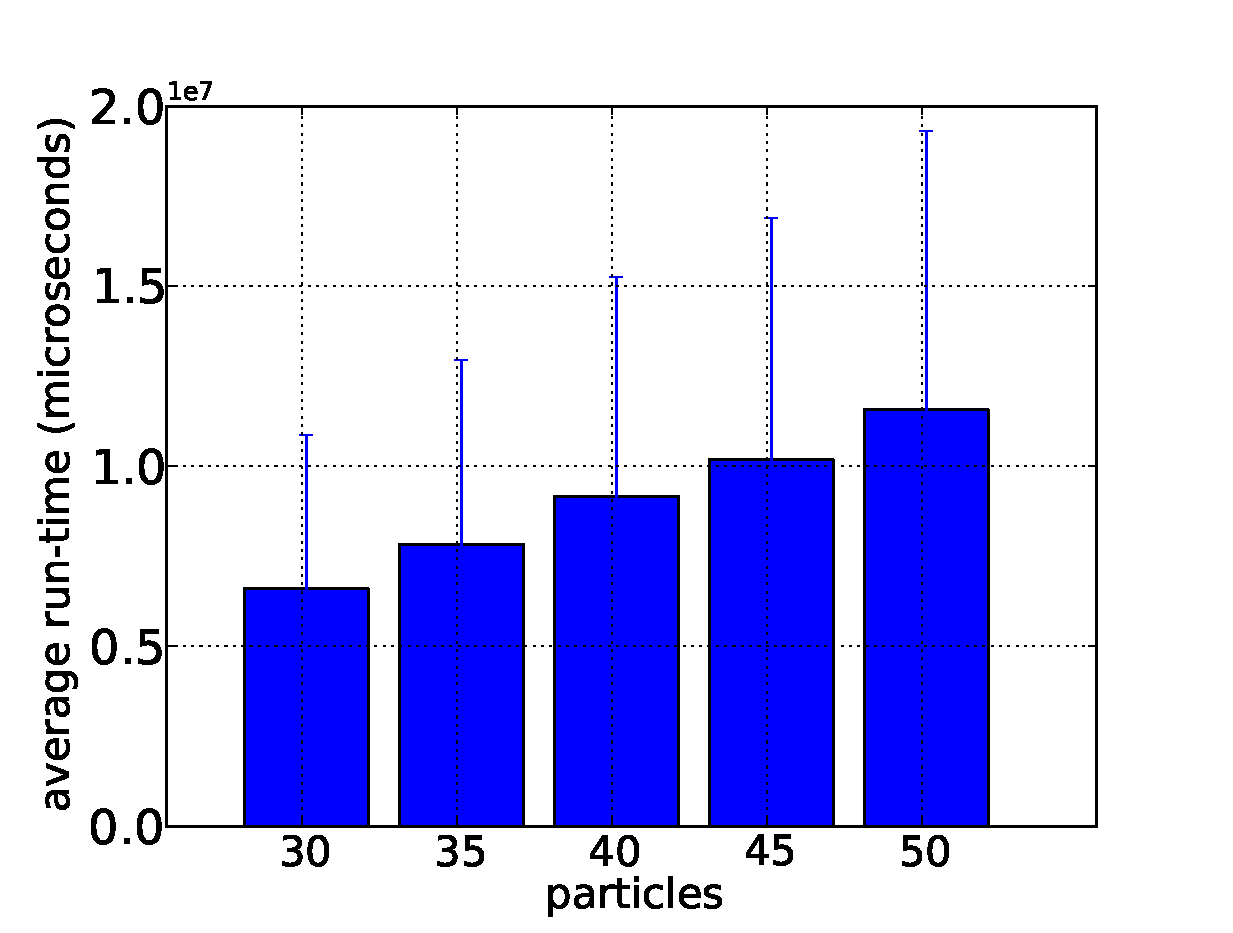
\includegraphics[width=0.45\columnwidth,keepaspectratio]{plot_fr-campus-20040714_carmen_log_Particles.eps}
 }
 \subfigure[3rd Floor of MIT CSAIL] {
 \centering
 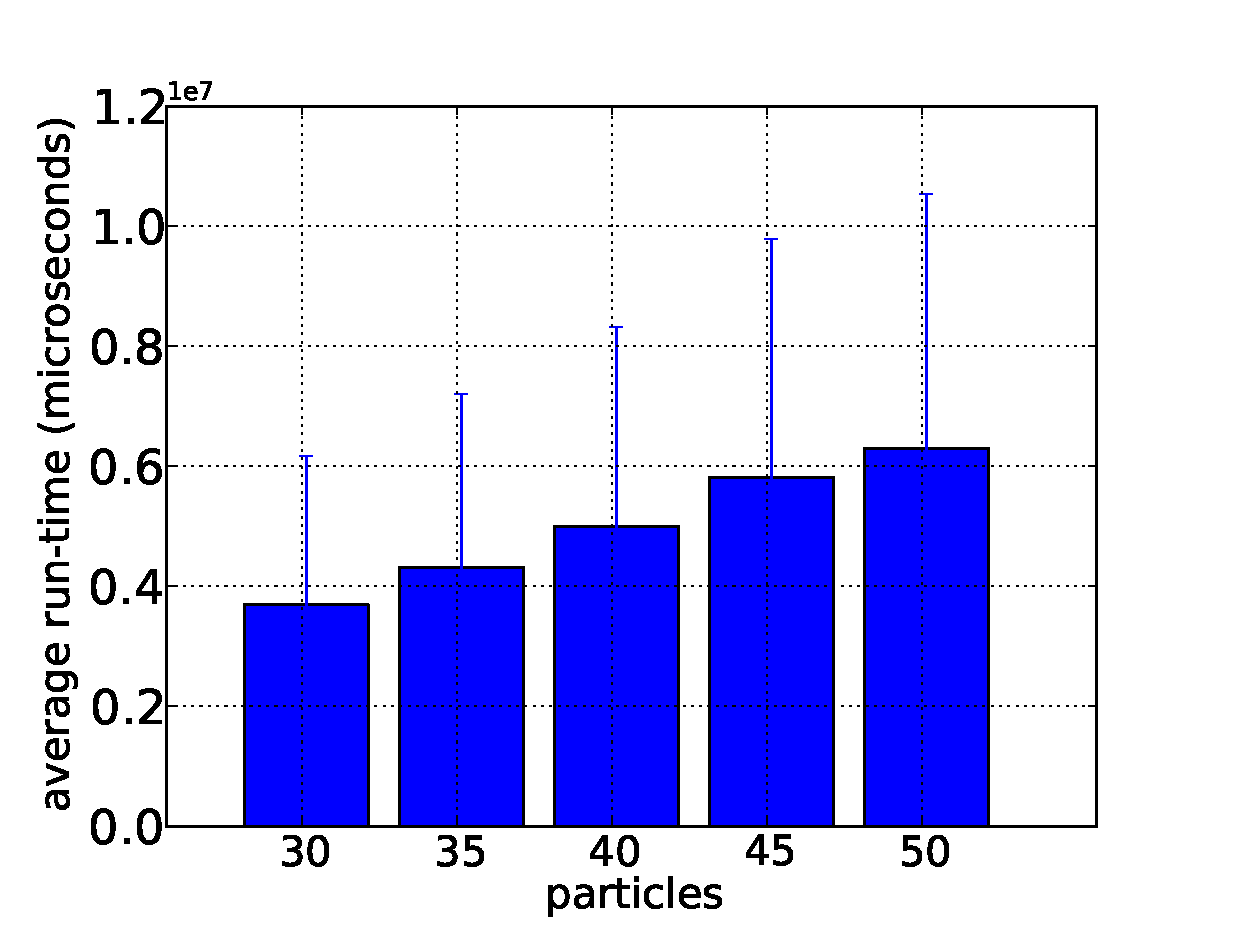
\includegraphics[width=0.45\columnwidth,keepaspectratio]{plot_mit-csail-3rd-floor-2005-12-17-run4_flaser_log_Particles.eps}
 }
 \subfigure[Edmonton Convention Centre] {
 \centering
 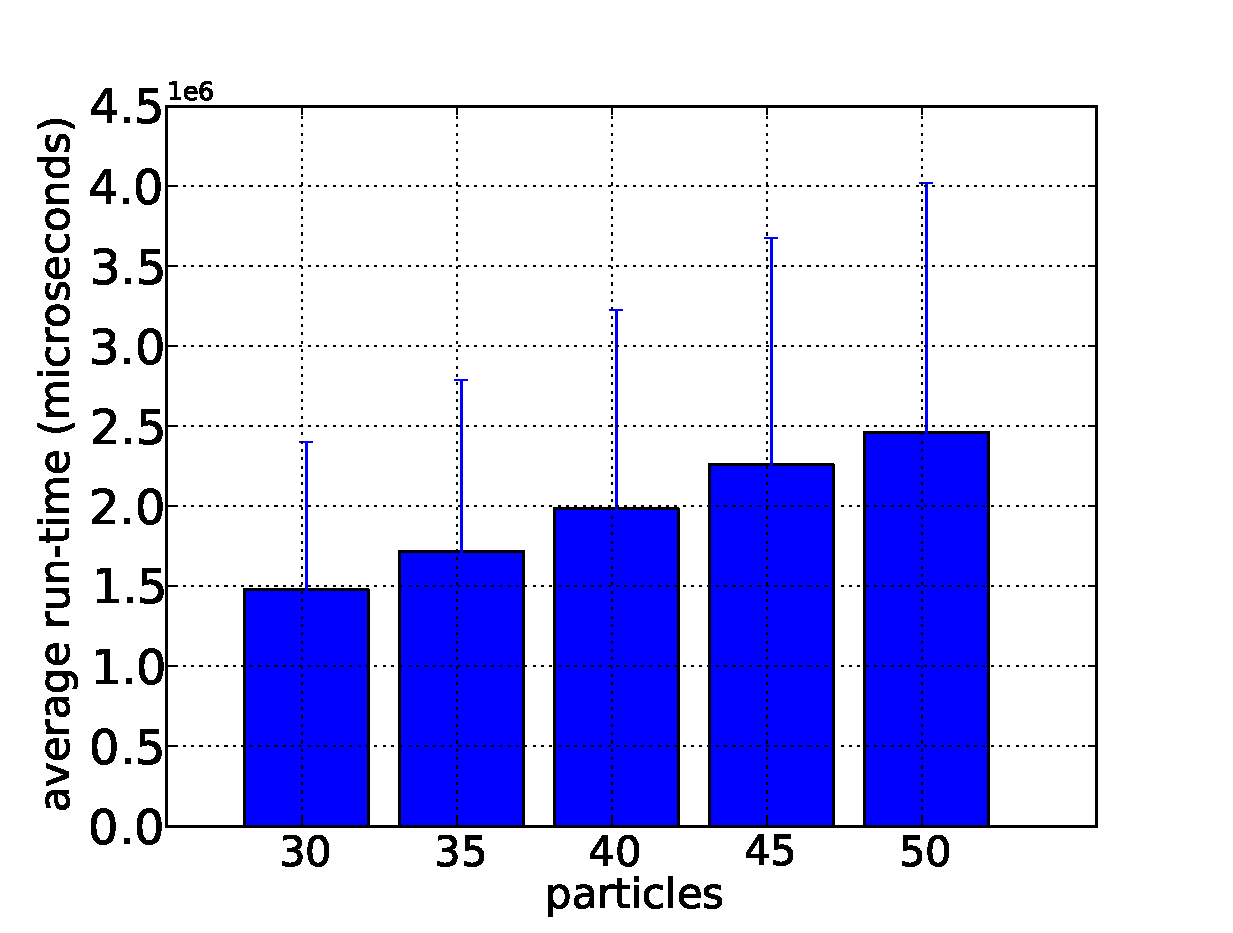
\includegraphics[width=0.45\columnwidth,keepaspectratio]{plot_edmonton_3_log_Particles.eps}
 }
 \caption{\FFD's run-time according to number of particles.}
 \label{fig:graph_ffd_run-time_vs_particle_numbers}
\end{figure}



\paragraph{Speeding-Up \WFD Even Further}\label{section:wfd_speedup}
\WFD's execution time can be boosted even more by
reducing the grid size (i.e., by using a coarse grid). Of course, there is a
trade-off between shorter execution time and the quality of the output frontiers. Even though, standard
exploration tasks can utilize the output frontiers received in this manner.
The grid is divided into blocks in size of the robot's width and height.
Smaller blocks will not make sure that robot will be able to pass through
terrain obstacles (i.e. corridors). Each block in the real world is represented
by a single cell in the reduced grid. In order to determine the occupancy value
of the cell, we examined different strategies. We considered both the speed of
creating the new grid and the quality of the output.
%such as: majority, average or
%sampling the certain cells in the block. 
We found out that sampling the center of the block edges and the
block center yields the best results. 
% \include{algorithms/iterative_frontier_detector_outline}
We plan to investigate efficient techniques to reduce the grid size while
considering the quality of the output coarse grid data. 
